\batchmode
\makeatletter
\def\input@path{{/Users/Adam/Dropbox/Stat215A-2013/Labs/Lab2/Lab//}}
\makeatother
\documentclass[english]{article}\usepackage{graphicx, color}
%% maxwidth is the original width if it is less than linewidth
%% otherwise use linewidth (to make sure the graphics do not exceed the margin)
\makeatletter
\def\maxwidth{ %
  \ifdim\Gin@nat@width>\linewidth
    \linewidth
  \else
    \Gin@nat@width
  \fi
}
\makeatother

\IfFileExists{upquote.sty}{\usepackage{upquote}}{}
\definecolor{fgcolor}{rgb}{0.2, 0.2, 0.2}
\newcommand{\hlnumber}[1]{\textcolor[rgb]{0,0,0}{#1}}%
\newcommand{\hlfunctioncall}[1]{\textcolor[rgb]{0.501960784313725,0,0.329411764705882}{\textbf{#1}}}%
\newcommand{\hlstring}[1]{\textcolor[rgb]{0.6,0.6,1}{#1}}%
\newcommand{\hlkeyword}[1]{\textcolor[rgb]{0,0,0}{\textbf{#1}}}%
\newcommand{\hlargument}[1]{\textcolor[rgb]{0.690196078431373,0.250980392156863,0.0196078431372549}{#1}}%
\newcommand{\hlcomment}[1]{\textcolor[rgb]{0.180392156862745,0.6,0.341176470588235}{#1}}%
\newcommand{\hlroxygencomment}[1]{\textcolor[rgb]{0.43921568627451,0.47843137254902,0.701960784313725}{#1}}%
\newcommand{\hlformalargs}[1]{\textcolor[rgb]{0.690196078431373,0.250980392156863,0.0196078431372549}{#1}}%
\newcommand{\hleqformalargs}[1]{\textcolor[rgb]{0.690196078431373,0.250980392156863,0.0196078431372549}{#1}}%
\newcommand{\hlassignement}[1]{\textcolor[rgb]{0,0,0}{\textbf{#1}}}%
\newcommand{\hlpackage}[1]{\textcolor[rgb]{0.588235294117647,0.709803921568627,0.145098039215686}{#1}}%
\newcommand{\hlslot}[1]{\textit{#1}}%
\newcommand{\hlsymbol}[1]{\textcolor[rgb]{0,0,0}{#1}}%
\newcommand{\hlprompt}[1]{\textcolor[rgb]{0.2,0.2,0.2}{#1}}%

\usepackage{framed}
\makeatletter
\newenvironment{kframe}{%
 \def\at@end@of@kframe{}%
 \ifinner\ifhmode%
  \def\at@end@of@kframe{\end{minipage}}%
  \begin{minipage}{\columnwidth}%
 \fi\fi%
 \def\FrameCommand##1{\hskip\@totalleftmargin \hskip-\fboxsep
 \colorbox{shadecolor}{##1}\hskip-\fboxsep
     % There is no \\@totalrightmargin, so:
     \hskip-\linewidth \hskip-\@totalleftmargin \hskip\columnwidth}%
 \MakeFramed {\advance\hsize-\width
   \@totalleftmargin\z@ \linewidth\hsize
   \@setminipage}}%
 {\par\unskip\endMakeFramed%
 \at@end@of@kframe}
\makeatother

\definecolor{shadecolor}{rgb}{.97, .97, .97}
\definecolor{messagecolor}{rgb}{0, 0, 0}
\definecolor{warningcolor}{rgb}{1, 0, 1}
\definecolor{errorcolor}{rgb}{1, 0, 0}
\newenvironment{knitrout}{}{} % an empty environment to be redefined in TeX

\usepackage{alltt}
\usepackage[T1]{fontenc}
\usepackage[latin9]{inputenc}
\usepackage{geometry}
\geometry{verbose,tmargin=1in,bmargin=1in,lmargin=1in,rmargin=1in}
\usepackage{fancyhdr}
\pagestyle{fancy}
\setlength{\parskip}{\smallskipamount}
\setlength{\parindent}{0pt}
\usepackage{amsthm}
\usepackage{amsmath}

\usepackage{wrapfig}
\usepackage{caption}
\usepackage{subcaption}
\usepackage[colorlinks,linkcolor=black,anchorcolor=blue,citecolor=black]{hyperref}

\makeatletter

%%%%%%%%%%%%%%%%%%%%%%%%%%%%%% LyX specific LaTeX commands.
\providecommand{\LyX}{L\kern-.1667em\lower.25em\hbox{Y}\kern-.125emX\@}

%%%%%%%%%%%%%%%%%%%%%%%%%%%%%% Textclass specific LaTeX commands.
\numberwithin{equation}{section}
\numberwithin{figure}{section}

\@ifundefined{date}{}{\date{}}
%%%%%%%%%%%%%%%%%%%%%%%%%%%%%% User specified LaTeX commands.
\pagestyle{empty} 

\makeatother

\usepackage{babel}
\begin{document}

\title{Lab 2 - Linguistic Survey\\
Stat 215A, Fall 2015}


\author{Ni,Wei; Pu,Qifan; Saha,Sujayam; Ye,Yuting}

\maketitle



\section{Introduction}
\label{sec:intro}
\qquad In this report, we studied the linguistic geography of the United States by analyzing the \textit{Harvard Dialect Survey} conducted in 2003. In Section~\ref{sec:data}, we performs data cleaning and preliminary data exploration. \textit{Question 74}, \textit{Question 76} and \textit{Question 86} are chosen for investigation. In Section~\ref{sec:dimred}, multi data reduction methods are applied to explore the dimensional characteristics of the dataset as well as to eliminate noise. The methods are \textit{Principal Component Analysis} (PCA)~\cite{pca}, \textit{Independent Component Analysis} (ICA)~\cite{ica} and \textit{Random Projection}~\cite{randomprojection}. In Section~\ref{sec:clustering}, we combine several clustering methods like \textit{k-means}~\cite{kmeans} clustering, \textit{Non-negative Matrix Factorization} (NMF)\cite{nmf}, \textit{k-medoids} clustering~\cite{kmedoids} and \textit{hierarchy} clustering~\cite{hierarchical} with data reduction methods on the linguistic data. The number of clustering is determined by gap statistics, average silhouette width and visualization. Four dialect regions are found after clustering, i.e., eastern part, middle part, southern part and western plus northern part of the U.S..  In Section~\ref{sec:stability}, we perturb the raw data by adding Gaussian noises in order to test the robustness the clustering method. We finally conclude in Section~\ref{sec:conc}. \textbf{Appendix} includes the kernel density portion from \textit{Lab1}.

%\section{The Data}
\section{The Data}
\label{sec:data}

\qquad There are 3 datasets provided, \textit{lingData}, \textit{lingLocation} and \textit{question\_data}. 47471 people from all over the country were surveyed on 122 questions, of which only 67 questions are used for our analysis. 
In dataset \textit{lingData}, each row is one individual with features \textit{ID}, \textit{CITY}, \textit{STATE}, \textit{ZIP}, \textit{lat} (latitude), \textit{long} (longitude) and their responses to questions. 
\textit{ID} is the individual index while \textit{CITY}, \textit{STATE}, \textit{ZIP}, \textit{lat}, \textit{long} describe the location. Dataset \textit{lingLocation} aggregates Dataset \textit{lingData} by put people with the same \textit{lat}, \textit{long} and responses together. Dataset \textit{question\_data} gives the concrete content of each question (Refer to \href{http://dialect.redlog.net/index.html}{Harvard Dialect Survey} for more questions).

\subsection{Data quality and cleaning}
\qquad We check the data quality and process some necessary data cleaning to make it tidy enough for further exploration and analysis. To figure out the geographic patterns of dialects, we decide to use \textit{county} as the basic unit with the belief that people in the same county are supposed to share the same cultures, customs and dialects. One way to assign each person to the county he locates in is to use \textit{FIPS county code}. We first need to match the \textit{ZIP code} offered in \textit{lingData} to \textit{FIPS county code} downloaded online. However, 5234 people's \textit{ZIP}s do not match any \textit{FIPS} approximately due to the incompleteness of our \textit{ZIP2FIP} file. We eventually decided to make use of each participant's \textit{lat} and \textit{long} to figure out his corresponding \textit{county}. During the procedure, we added another two fields to each individual, \textit{COUNTY} (merging both the state and the county by ',') and \textit{group} (the index of \textit{COUNTY}). The following are steps of data cleaning:

\begin{enumerate}
\begin{figure}[t!]
    \centering
    \begin{subfigure}[t]{0.49\textwidth}
        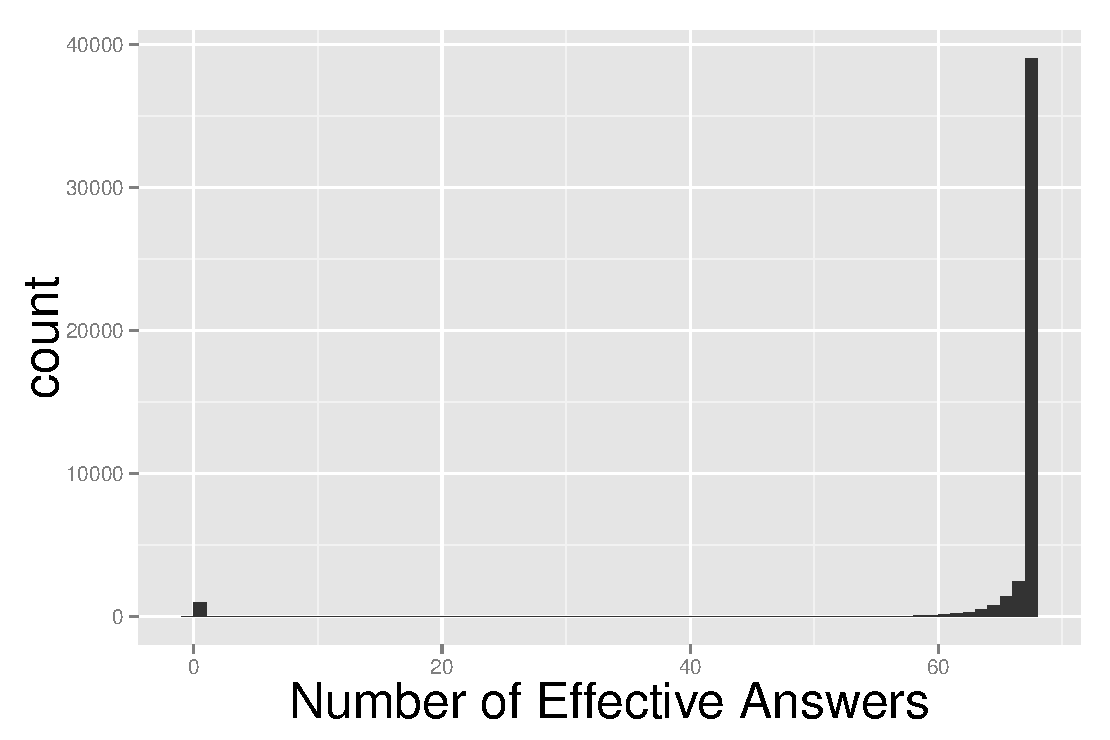
\includegraphics[width=1\textwidth]{fig/Anw_distri_all.pdf}
        \caption{all}
    \end{subfigure}
    \begin{subfigure}[t]{0.49\textwidth}
        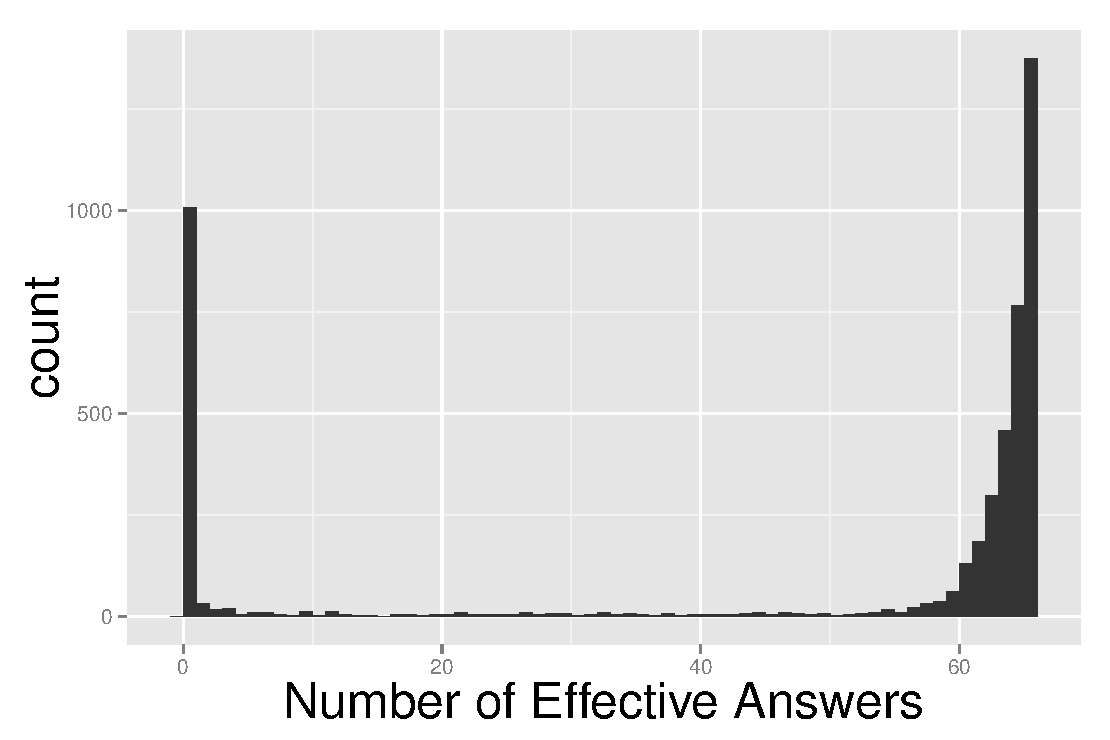
\includegraphics[width=1\textwidth]{fig/Anw_distri_65.pdf}
                \caption{no more than 65}
    \end{subfigure}
    \caption{\textbf{The distribution of people with different numbers of effective responses.} \textbf{(a)} All people. \textbf{(b)}  People who had no more than 65 responses.} 
\end{figure}

\item Our focus is on the mainland of the U.S., thus areas outside the American mainland are excluded, like Alaska, Hawaii. In this step, 1232 people are not in the range. There remain 46239 individuals.

\item There are some missing responses for a few people due to erroneous records or that they were not willing to response the corresponding question. People with few responses are of little use to our analysis, thus need to be excluded. After having a look at the distribution of people with different effective responses (See \textbf{Figure xxx}), we selected people who had responded to at least 60 questions, with little loss of information. In this step, there remain 44683 people.

\item As mentioned above, each individual's county is figured out by using their \textit{lat} and \textit{long}. However, some people cannot be matched to any counties, thus should be removed from the datasets. During the matching process, we add both the name of count (\textit{COUNTY}) and the county index (\textit{group}) each person. In this step, there remain 43401 people.

\item Some counties have more than one count indexes, which may be used to differentiate the direction of counties, e.g. North Berkeley and South Berkeley. Without much loss of information, we remove such repetitions. In this step, there remain 43266 people.

\item Since the question response belongs to categorical data and cannot be compared directly between questions. We need to transform each person's response into a binary format. For example, if one question has 4 responses one person chose the second option, his response is expressed as $(0,1,0,0)$. Finally, each person has a response vector of length of 468 (the sum of the number of responses times the number of its associated options), each loading is an indicator if he chose this option. Here we get a response matrix with dimension of 43266 by 468 on individual level.

\item We also aggregate the response matrix on individual level into county level with the consideration that the county is our basic unit for dialect geography. We simply take an average of the response vectors among people in the same county. The dimension of the response matrix on county level is 2362 by 468. 

\end{enumerate}

\begin{figure}[t!]
    \centering
    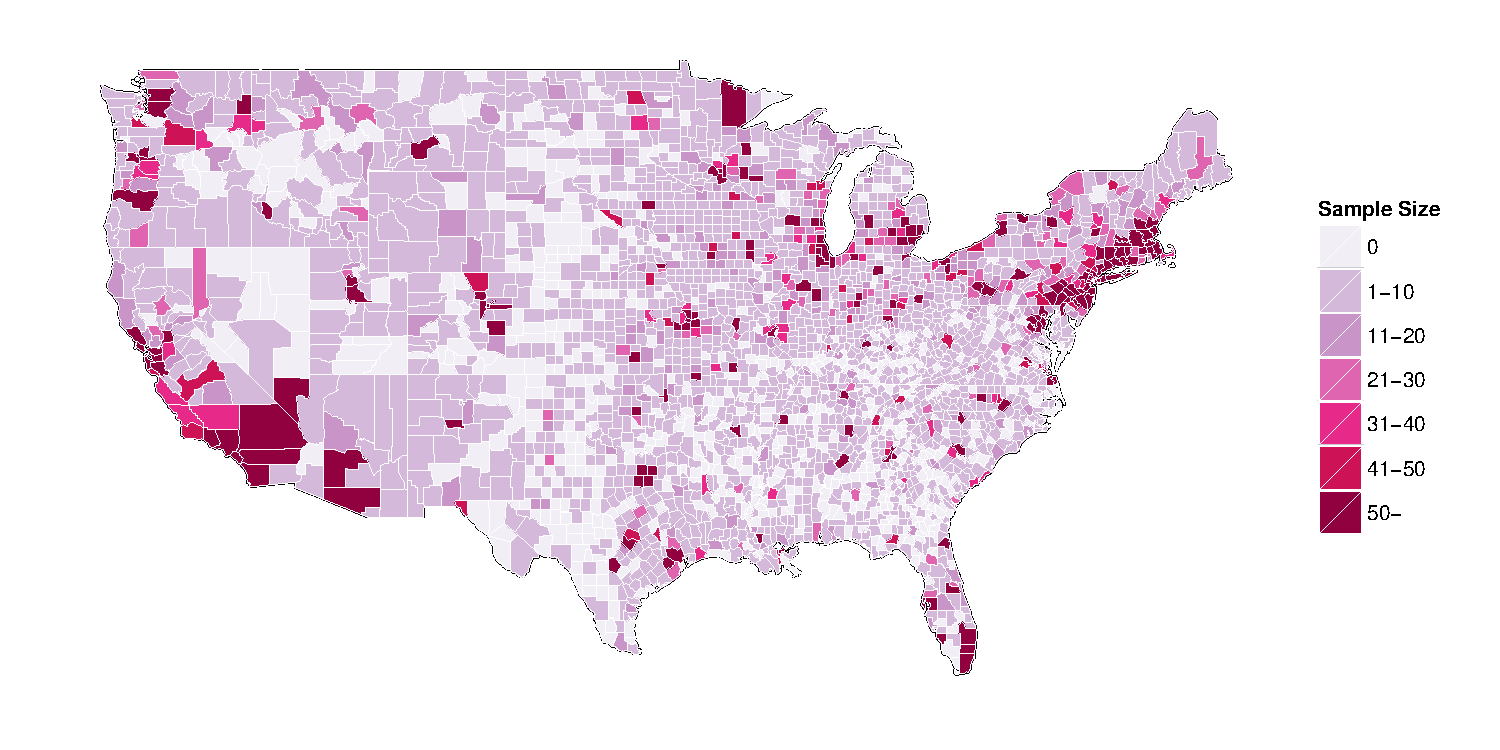
\includegraphics[width=1\textwidth]{fig/Map_size.pdf}   
    \caption{\textbf{The distribution of sample size on counties} 2362 counties have people who taken part in the survey while 713 counties have no surveyed individuals.} 
\end{figure}

\qquad We only make use of Dataset \textit{lingData} and match the counties by ourselves in case of the inaccuracy of the existing \textit{CITY} and \textit{ZIP} information. The data possesses high quality so that we do not make too many efforts for tidying it. But the survey design receives the doubt that people were not surveyed uniformly from all over the countries. 713 counties do not have people who taken part in the survey (See \textbf{Figure xxx}).


\subsection{Exploratory Data Analysis}

\qquad To figure out if there are any questions that can determine the dialect geography patterns, we pick out 3 questions to look into, i.e. \textit{Question 74}, \textit{Question 76} and \textit{Question 89}. The contents are displayed as followings: 

\begin{itemize}
\item Q074: What do you call the little gray creature (that looks like an insect but is actually a crustacean) that rolls up into a ball when you touch it?
   
\item Q076:  What term do you use to refer to something that is across both streets from you at an intersection (or diagonally across from you in general)?

\item Q089: Can you call coleslaw "slaw"?
\end{itemize}

\qquad These three questions focus on the way people call several common stuffs. \textit{Question 74} has 14 choices, \textit{Question 76} has 9 and \textit{Question 89} has 5, which reflects the diversity of dialects. \textit{Question 76} and \textit{Qeustion 89} share a similar pattern that they separate the southern interviewees from the others, while \textit{Question 74} isolates the northern part and eastern part (See \href{https://yeyt2718.shinyapps.io/map_Question}{Map Set} for the map distribution based on questions). It's easy to interpret the isolated eastern and northern part with responses like 'no idea' as the cold environment offer them few opportunities of seeing such bugs. But other questions may involve complicated cultural and historical factors.\\




\qquad  We further try to find out if there exists obvious association between different questions. The correlation of the pairwise questions is calculated by performing a kernel density estimation on the two dimension distribution (e.g., $Q074 \times Q076$), as shown in \textbf{Figure \ref{fig:question distribution}}. Most people incline to response 'roly poly' to \textit{Question 74} and 'kitty-conner' to\textit{Question 76} simultaneously or take 'roly poly' and 'catty corner' as a pari. Such connection can help predict the response for each other. No meaningful information can be extracted by looking at the 2D density estimation between \textit{Question 74} and \textit{Question 89} or between \textit{Question 76} and \textit{Question 89}. It just indicates that we should not only focus one or two questions to detect the dialect geography, but should aggregate all of them for analysis \textbf{[reference!]}. Motivated by this, we move on implementing clustering methods based on all the 67 questions.



\begin{figure*}[t!]
%  \begin{minipage}[b]{0.49\textwidth}
%    \centering
%    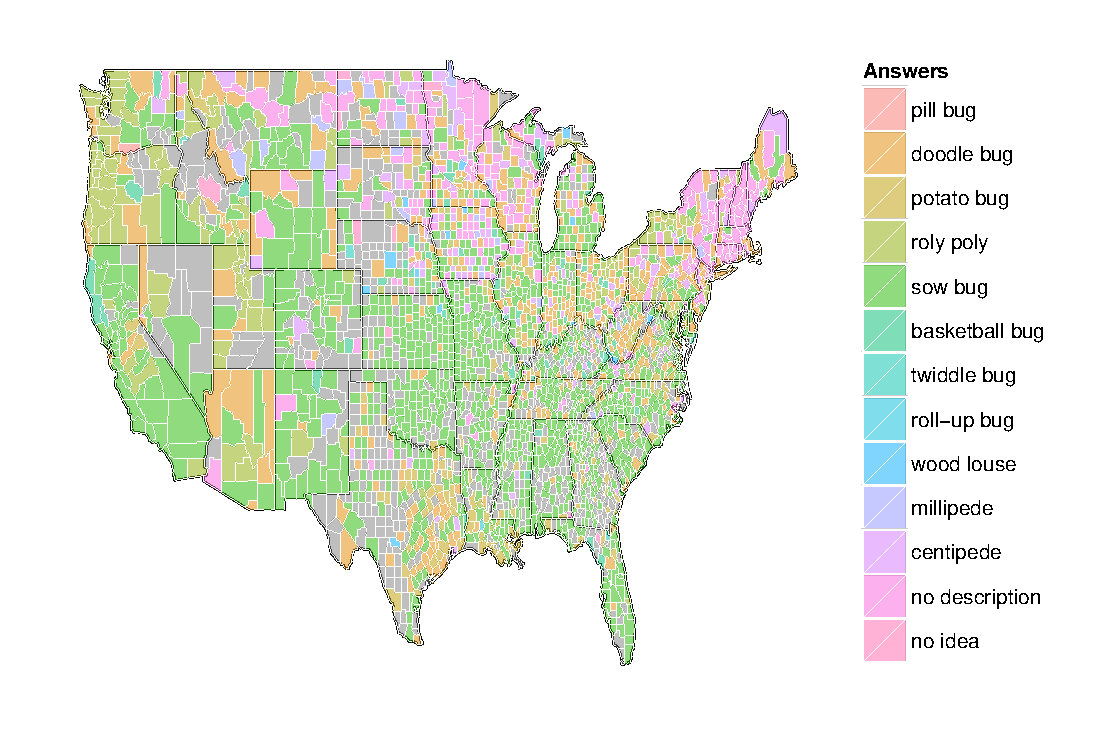
\includegraphics[width=1.1\columnwidth,height=0.7\columnwidth]{fig/Map_Q74.pdf}
%    \subcaption{Question 74}\label{subfig:hierarchy1}
%  \end{minipage}
  \begin{minipage}[t]{0.33\textwidth}
    \centering
    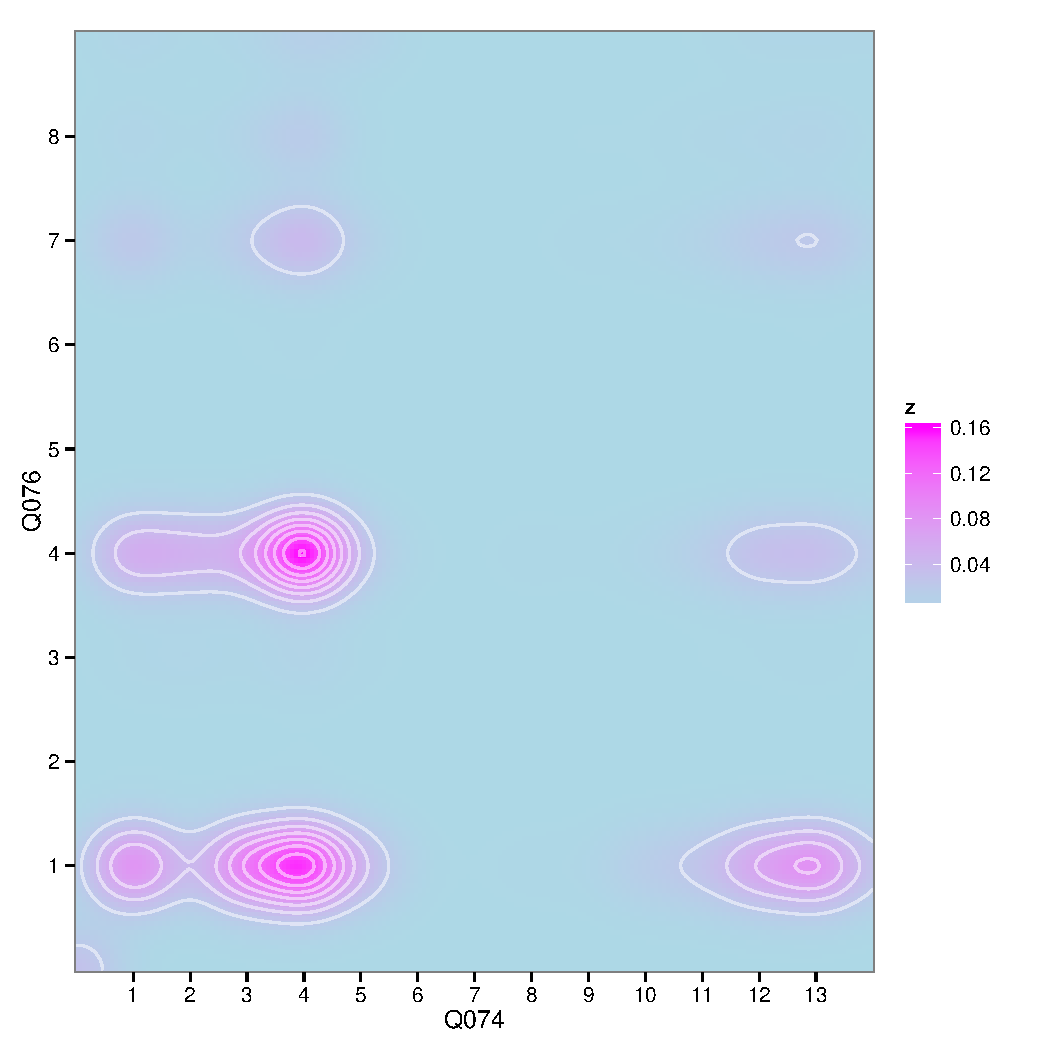
\includegraphics[width=\columnwidth,height=0.8\columnwidth]{fig/2dhist_q074_q076.pdf}
    \subcaption{Q074 and Q076}\label{subfig:hierarchy2}
  \end{minipage}
%  \begin{minipage}[b]{0.49\textwidth}
%    \centering
%    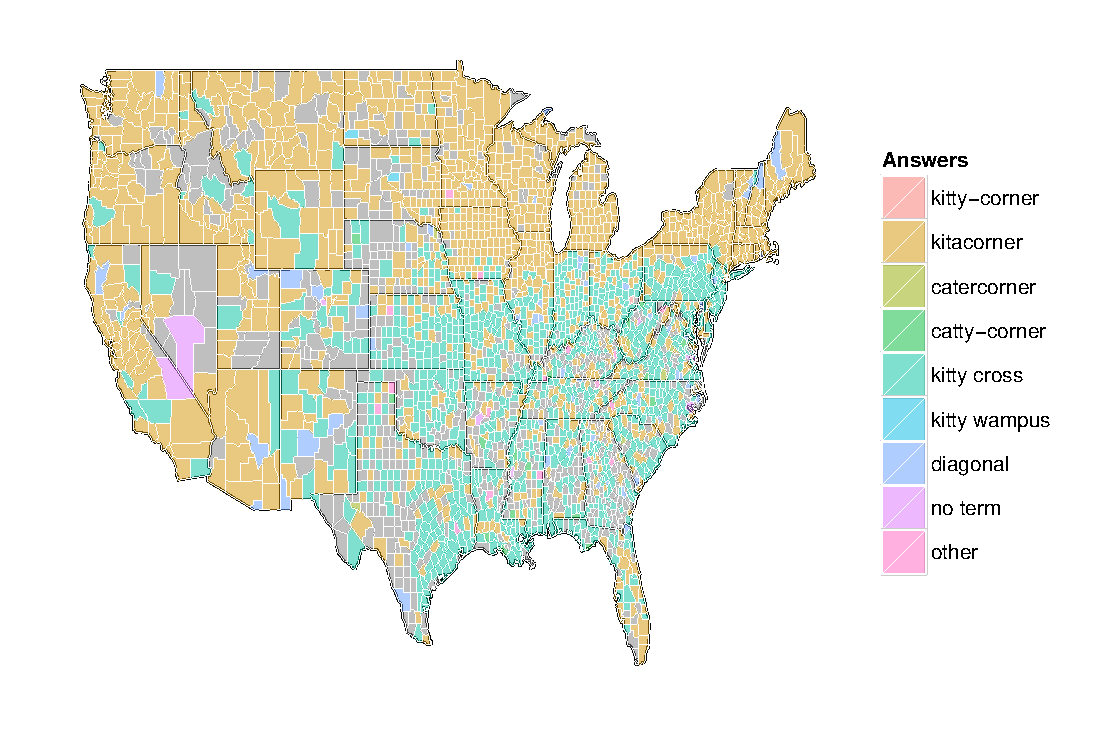
\includegraphics[width=1.1\columnwidth,height=0.7\columnwidth]{fig/Map_Q76.pdf}
%    \subcaption{Question 76}\label{subfig:hierarchy3}
%  \end{minipage}
  \begin{minipage}[t]{0.33\textwidth}
    \centering
    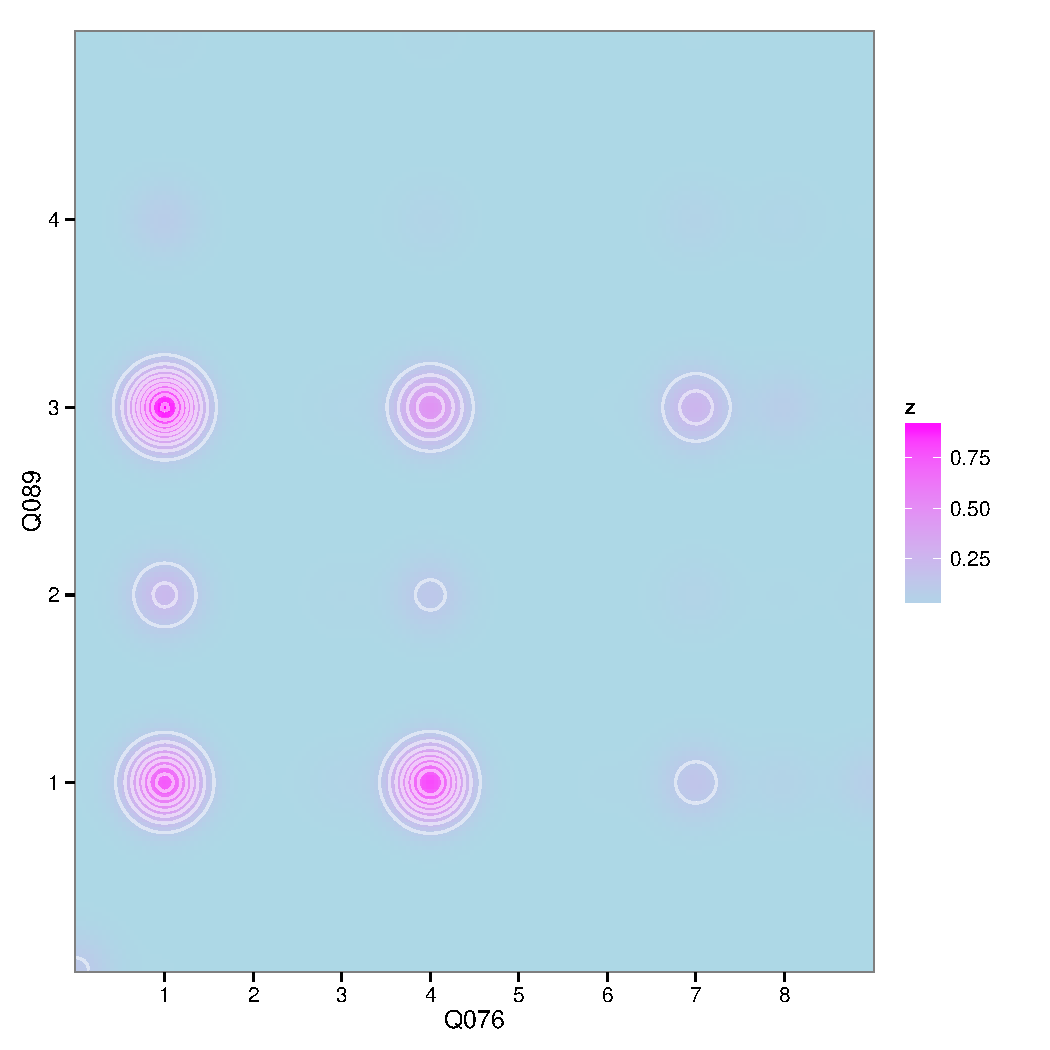
\includegraphics[width=\columnwidth,height=0.8\columnwidth]{fig/2dhist_q076_q089.pdf}
    \subcaption{Q076 and Q089}\label{subfig:hierarchy4}
  \end{minipage}
%  \begin{minipage}[b]{0.49\textwidth}
%    \centering
%    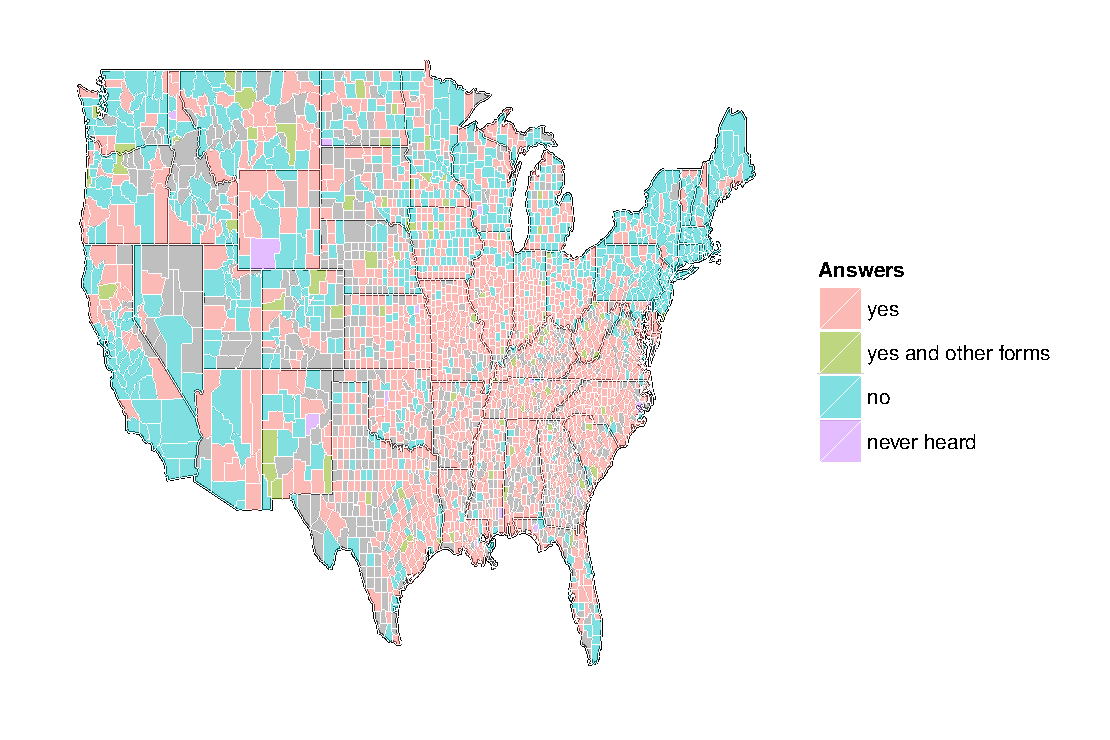
\includegraphics[width=1.1\columnwidth,height=0.7\columnwidth]{fig/Map_Q89.pdf}
%    \subcaption{Question 89}\label{subfig:hierarchy6}
%  \end{minipage}
  \begin{minipage}[t]{0.36\textwidth}
    \centering
    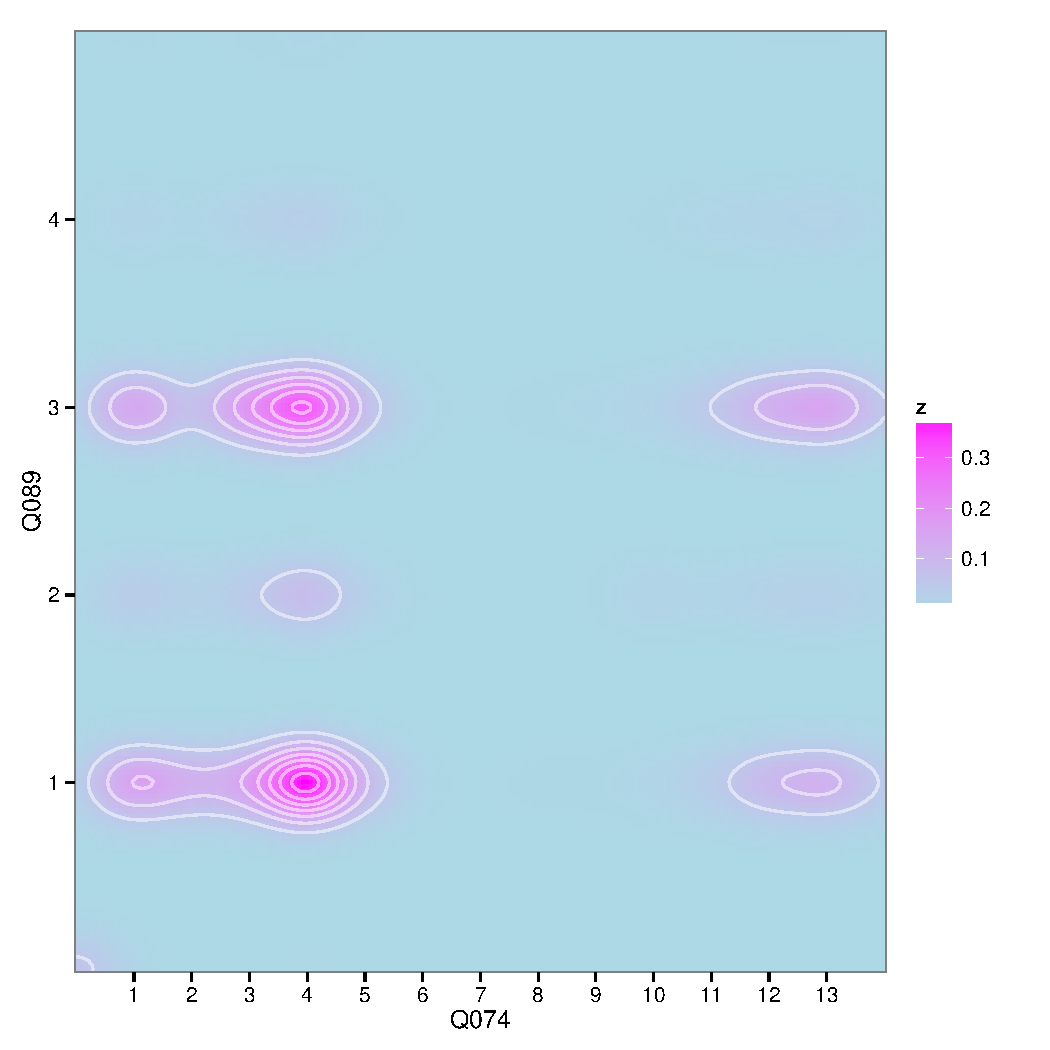
\includegraphics[width=\columnwidth,height=0.8\columnwidth]{fig/2dhist_q074_q089.pdf}
    \subcaption{Q074 and Q089}\label{subfig:hierarchy}
  \end{minipage}
  \caption{\textbf{Pairwise 2D Kernel densitiy estimation.}}
  \label{fig:question distribution}
\end{figure*}


%\begin{figure}[t!]
%    \centering
%    \begin{subfigure}[t]{0.49\textwidth}
%        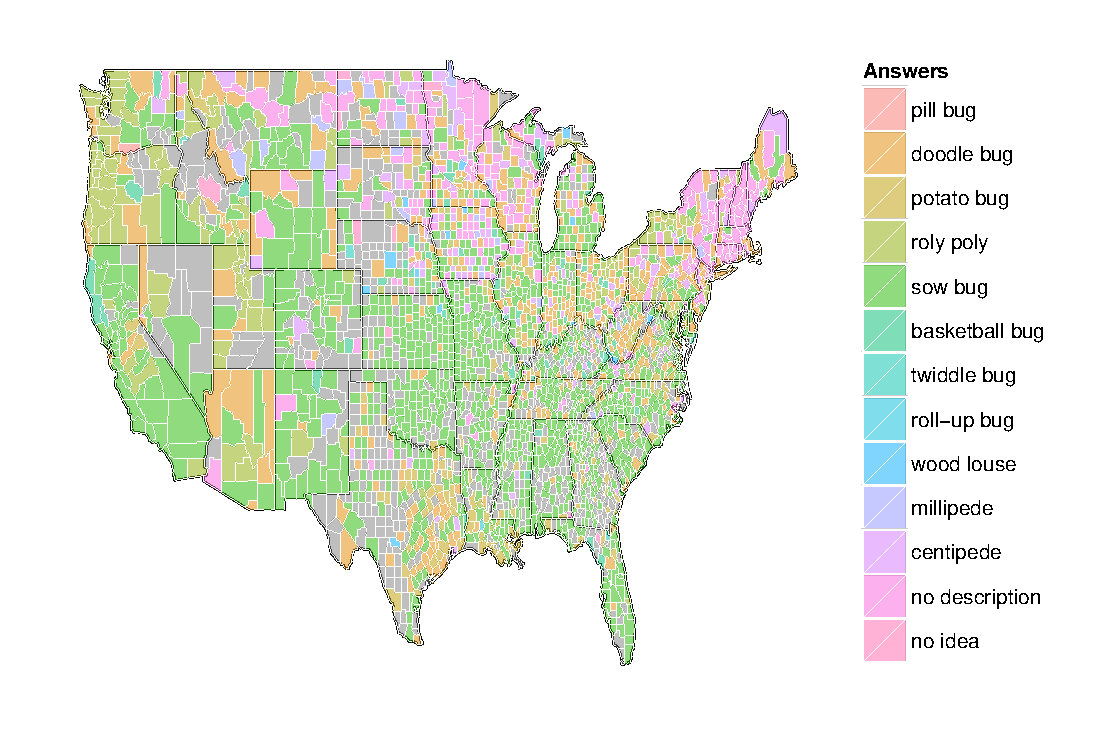
\includegraphics[width=1.1\textwidth]{fig/Map_Q74}
%        \caption{Question 74}
%    \end{subfigure}
%    \begin{subfigure}[t]{0.49\textwidth}
%        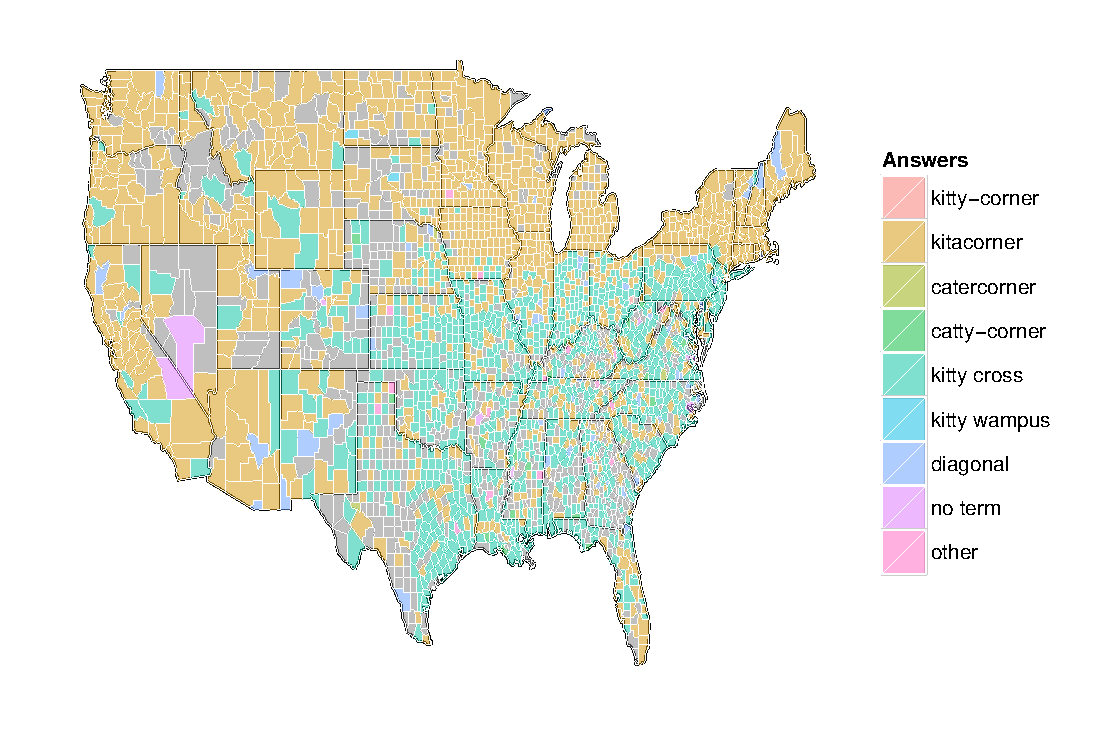
\includegraphics[width=1.1\textwidth]{fig/Map_Q76}
%        \caption{Question 76}
%    \end{subfigure}
%    \caption{\textbf{Answer distribution} \textbf{(a)} Q74. \textbf{(b)} Q76.} 
%\end{figure}

%\noindent In order to quantify the correlation of the two questions (Q074 and Q076), we performed a %kernel density estimation on
%the two dimension distribution ($Q074 \times Q076$), as shown in Figure xx. One see a clear %correlation from the heatmap plotting.\\

%\begin{figure}
%\centering
%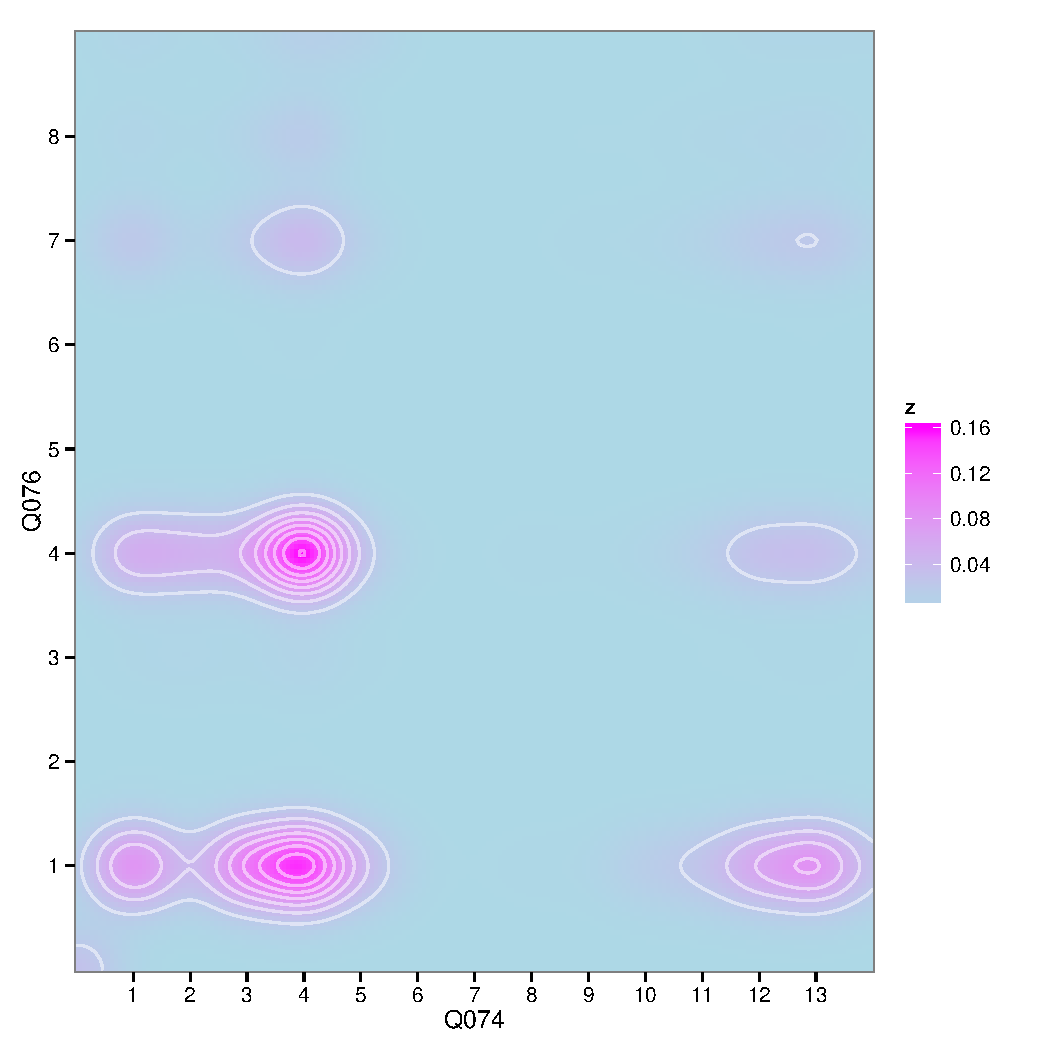
\includegraphics[width=0.45\linewidth]{fig/2dhist_q074_q076}
%\caption{Kernel density estimation for Q074 and Q096}
%\end{figure}

%\noindent Considering more then two questions, we involved Q089, which also share a similar trend %with Q076 and Q074. See Figure xx for the distribution of Q089. And also, we plot two-dimensional %kernel density estimation for two pairs (Q076 vs Q089, Q074 vs Q089), as shown in
%Figure xx.

%\begin{figure}
%\centering
%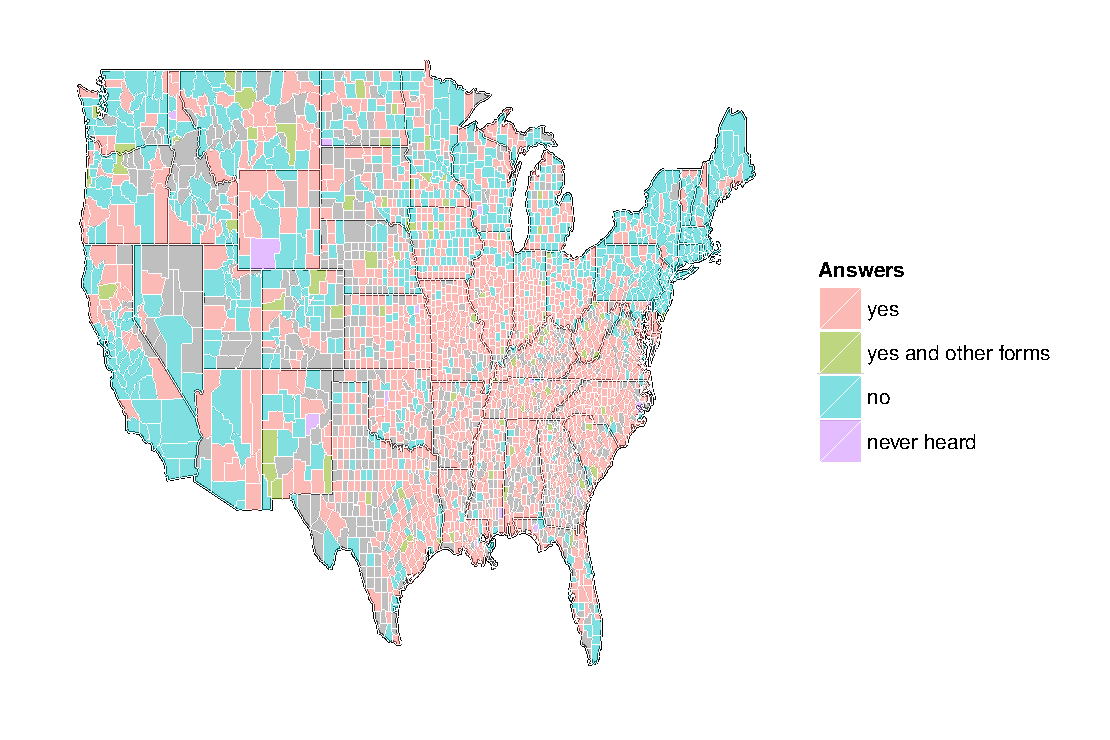
\includegraphics[width=0.9\linewidth]{fig/Map_Q89}
%\caption{Answer Distribution for Q089}
%\end{figure}


%\begin{figure}[t!]
%    \centering
%    \begin{subfigure}[t]{0.49\textwidth}
%        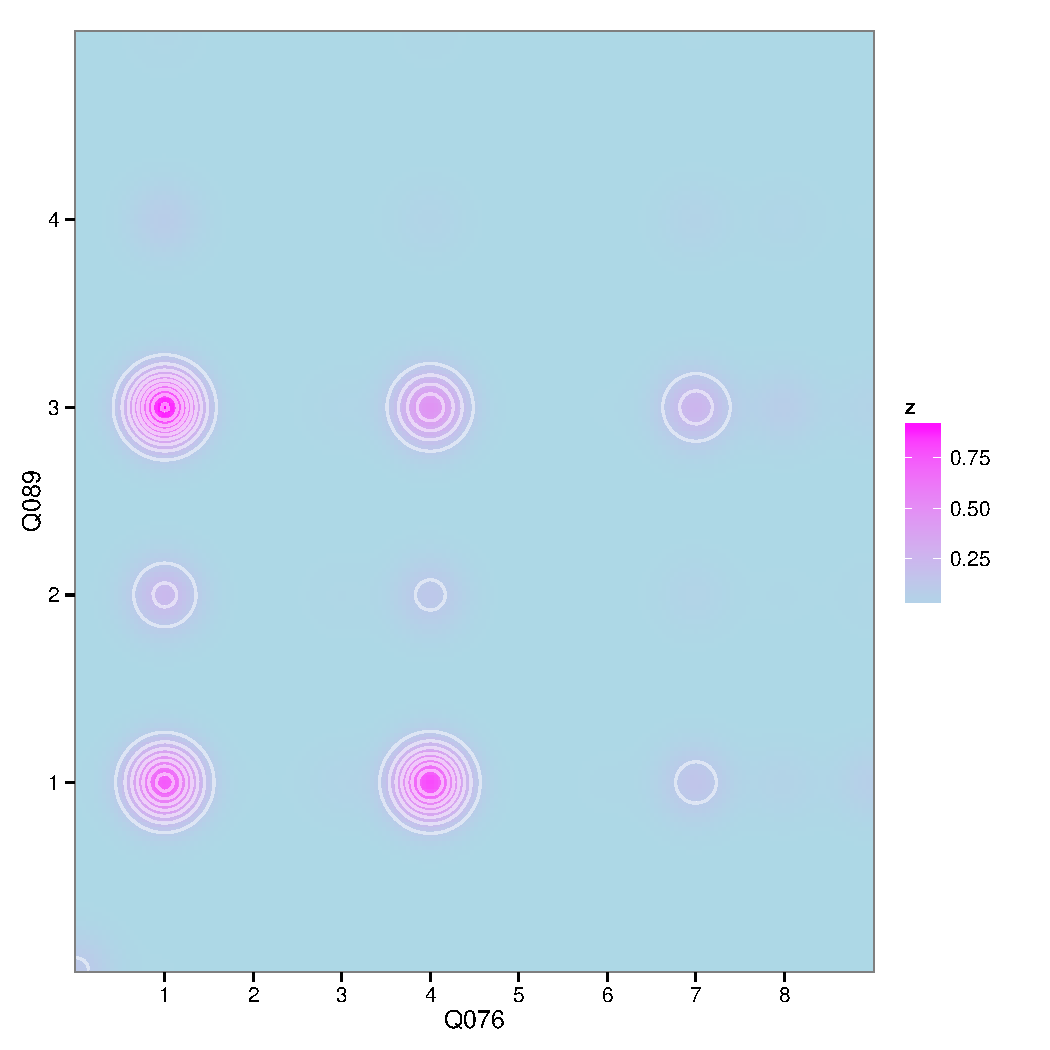
\includegraphics[width=1.1\textwidth]{fig/2dhist_q076_q089}
%        \caption{Q076 .vs. Q089}
%    \end{subfigure}
%    \begin{subfigure}[t]{0.49\textwidth}
%        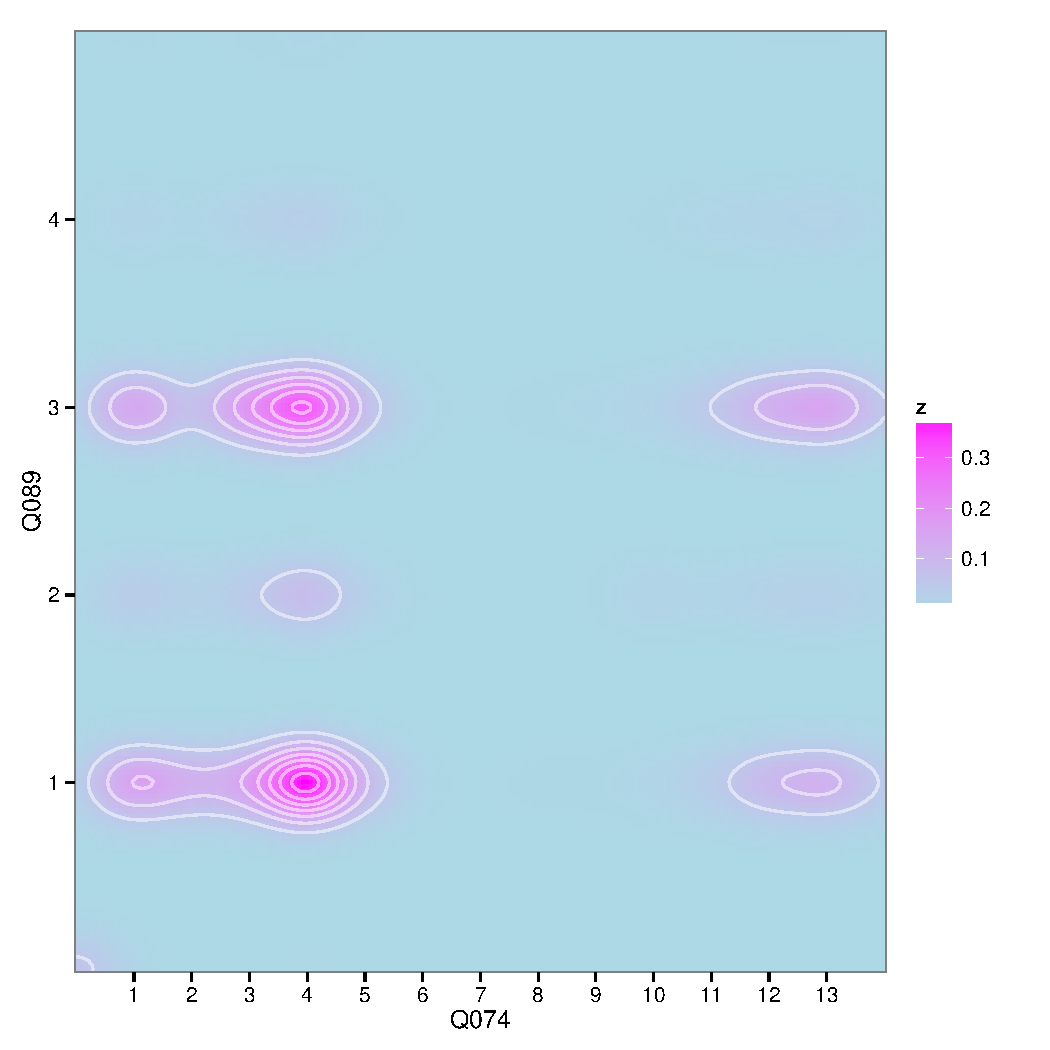
\includegraphics[width=1.1\textwidth]{fig/2dhist_q074_q089}
%        \caption{Q074 .vs. Q089}
%    \end{subfigure}
%    \caption{\textbf{Kernel Density Estimation} \textbf{(a)} Q76 .vs. Q089 \textbf{(b)} Q74 .vs. %Q089} 
%\end{figure}


%\section{Dimension Reduction Methods}
\section{Dimension Reduction}
\label{sec:dimred}

In the previous section we created a $43266 \times 468$ matrix containing binary values encoding the survey responses of all individuals. Let us denote this matrix \verb|mat|. In the rest of this analysis our goal is to extract information about how these individuals can be clustered into groups based on their dialects. It is often cumbersome and opaque to work in a space of $468$ dimensions and further it is unlikely that all $468$ variables are actually important in the questions we are trying to answer. To this end we shall in this section we investigate various dimension reduction techniques. Our goal is to reduce the ambient dimension from $468$ to a manageable number.

In investigating various methods of dimension reduction and comparing them against each other, we need to decide on how to compare clusterings. For instance let $c^1$ and $c_2$ denote two possible clusterings of $n$ data points (in this case, $n = 43266$ individuals). That is, $c^1_i$ is an integer denoting the cluster to which $i^{th}$ individual has been allocated in the first clustering. We could of course visualize both clusters in separate plots (how to do this is still a question since we are sitting in a large dimensional space), and then visually inspect how close they are. But this requires human intervention and is both time-consuming and subjective.

Instead, we use the notion of Rand index \cite{randindex} to compute the similarity of two clusterings. Rand index can be defined using the following expression,
$$
R(c^1,c^2) = \frac{a+b}{{n \choose 2}}
$$
where $a$ is the number of pairs of individuals who are clustered together in both $c^1$ and $c^2$ and $b$ is the number of pairs of individuals who are clustered separately in both $c^1$ and $c^2$. Note that the denominator is simply the total number of pairs of individuals. In the above definition the number of clusters in $c^1$ and $c^2$ need not be same. Mathematically, the Rand index can be written as below, where for a set $S$, its cardinality is denoted by $|S|$, and the $i^{th}$ individual is dentoed by $x_i$,
$$
R(c^1,c^2) = \frac{|\{(i,j)|c^1_i = c^1_j, c^2_i = c^2_j \}| + |\{(i,j)|c^1_i \neq c^1_j, c^2_i \neq c^2_j \}|    }{{n \choose 2}}
$$

It can be observed that $0 \leq R \leq 1$ always and $R = 1$ iff the two clusterings are equivalent.

In the following subsections, we begin computing various sketched versions of \verb|mat|. In order to judge the performance of such reductions, we can and will use some visual inspection. But, to get more quantified results, we will use the following scheme: let \verb|reducedmat| denote a sketch of \verb|mat| produced by a generic dimension reduction technique. We will compute k-means clusterings based on both the full data \verb|mat| and the reduced data \verb|reducedmat| and compare the similarity of these two clusterings via Rand index.

For this analysis, we will primarily fix $k=4$. This number is arrived at by gap statistic analysis and visual inspection of the result of k-means on full data. More details on this are forthcoming in later sections.

\subsection{Principal Component Analysis}

The first technique we shall investigate is PCA. To decide on the number of PC's, we gather all principal components and their variance from \verb|mat|. The variances and cumulative variances of the principal components are shown in Figure \ref{fig:pcvars}.

\begin{figure}[ht]
	\centering
	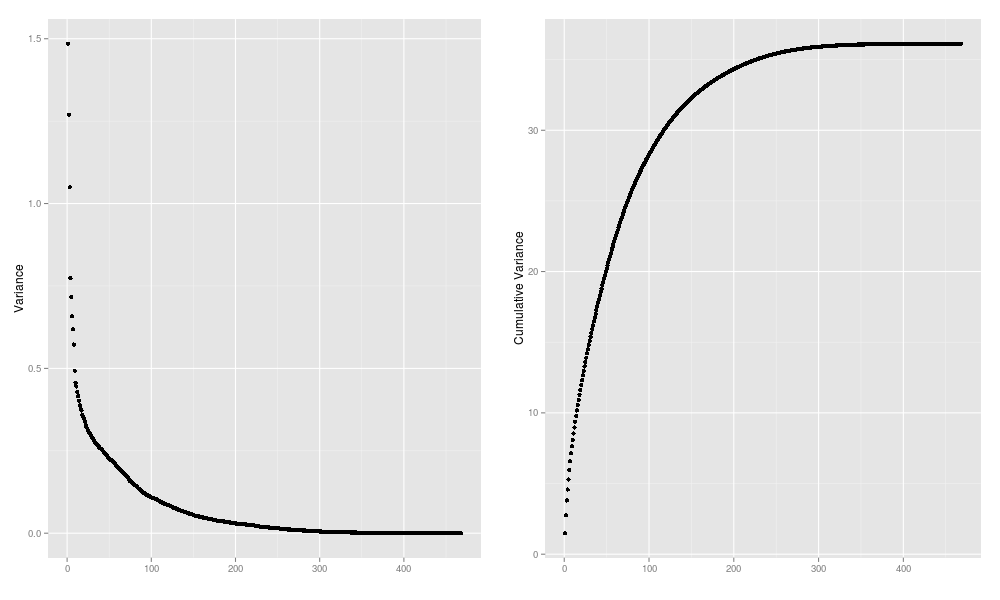
\includegraphics[width=0.8\textwidth]{fig/plot1.png}
	\caption{Variance and Cumulative Variance of Principal Components}
	\label{fig:pcvars}
\end{figure}


\begin{figure}[ht]
	\centering
	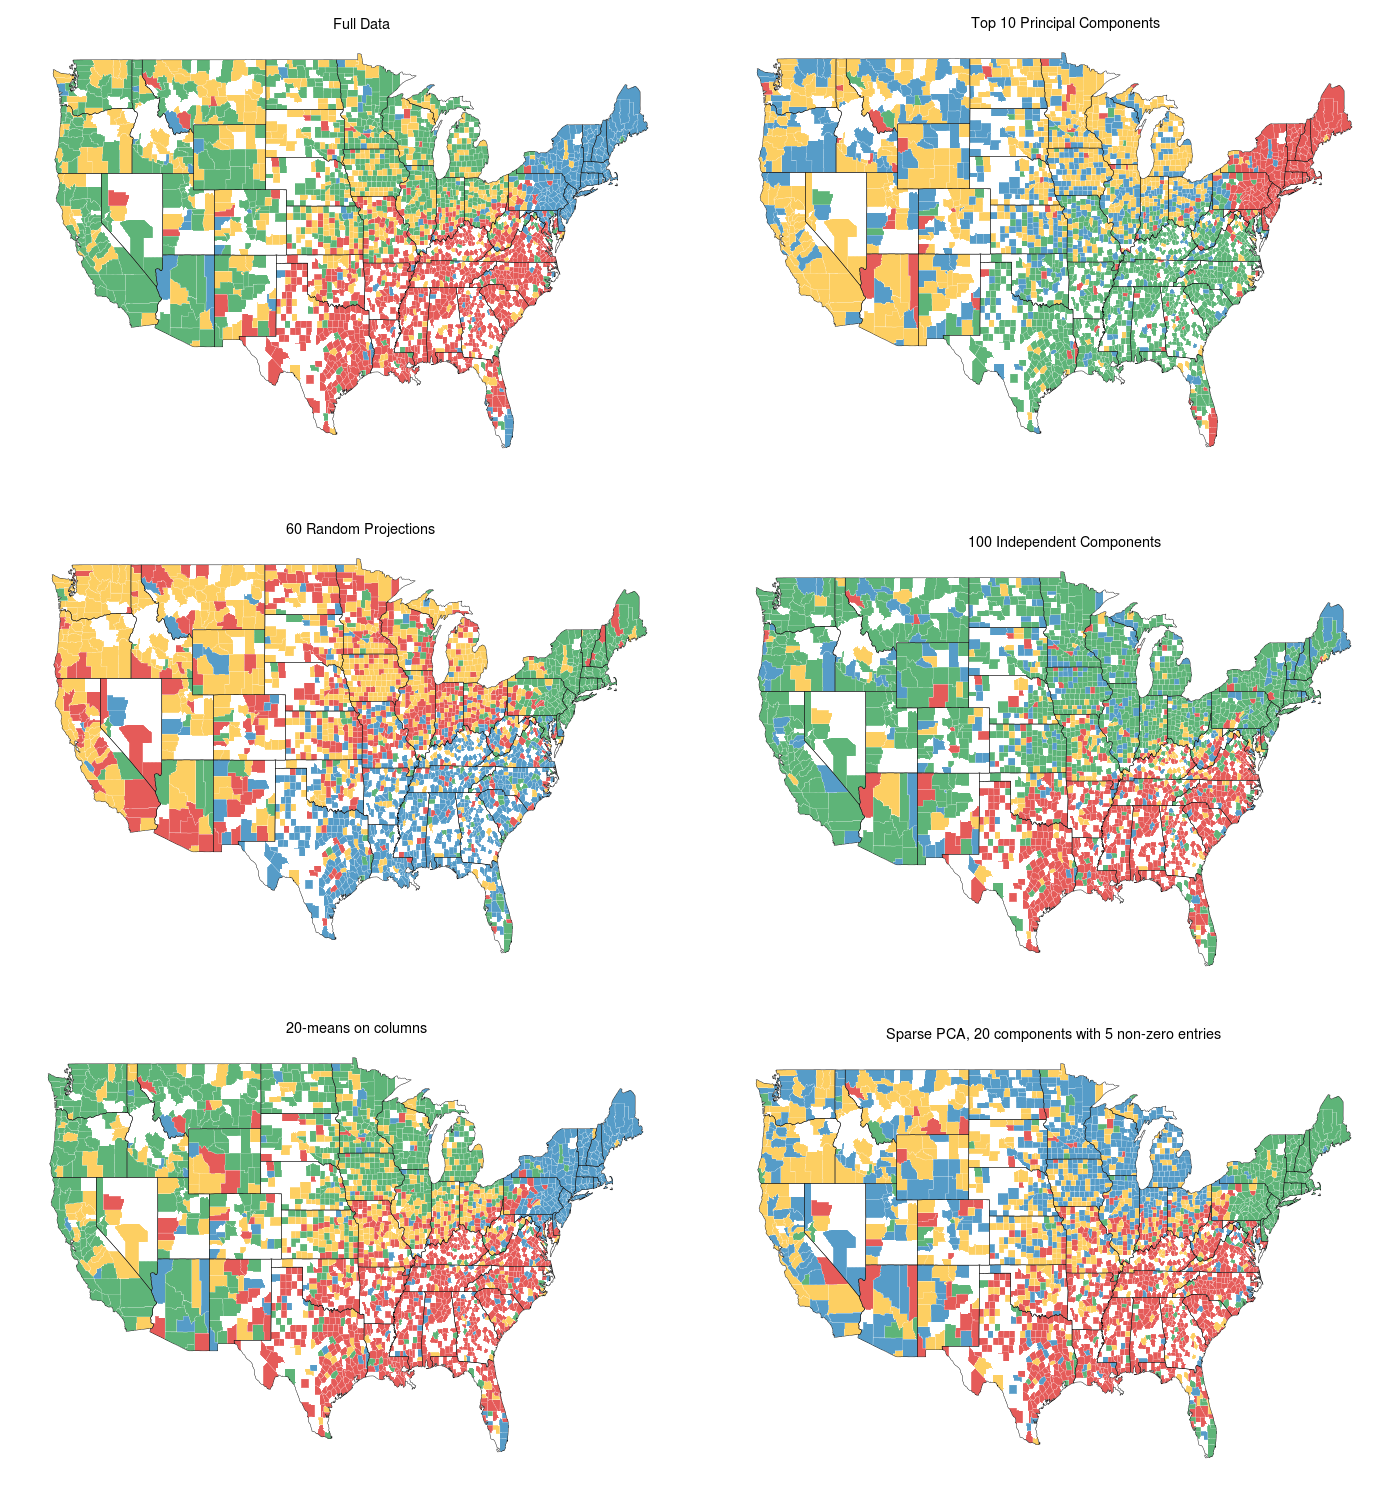
\includegraphics[width=0.8\textwidth]{fig/plot2to6.png}
	\caption{Comparison of 4-means clustering results on full data and various dimension reduction approaches. From top left in row major order: Full data, top $10$ principal components,}
	\label{fig:allplots}
\end{figure}

Observe that, the principal components do not show a sharp dropoff in variance, indicating that there is no small dimensional linear subspace which contains almost all of the variance in \verb|mat|. Dimension reduction by PCA is not likely to be very helpful in this data since we will need a lot of principal components in order to capture the full shape of the data.

Next we compute the k-means output of full data and top $10, 50, 100, 150, 200$ principal components. To save space for more interesting visualizations later in the document, we refrain from including the output visually at this point. We can compare the Rand index at each level of reduction. It is found that the Rand indices are \verb|0.96 0.99 0.84 0.80 0.80|. This makes using the top $10$ PC's quite desirable even though they explain only $20\%$ of the variance of the data. Note that the Rand indices are inherently random since the initial point of $k$-means algorithm is random. We shall revisit this consideration later. But this leads us to our next discussion. Fixing the number of principal components apriori does not tell us how much of the original variability in the data has been captured by the data. In the next sequence of plots, we investigate with top PC's chosen so that they explain $50\%, 80\%$ and $90\%$ of the data (the number of PC's required are $42, 106$ and $155$ respectively). In this case, the Rand indices come out as \verb|0.94 0.99 0.93|, further indicating that
\begin{center}
\verb|mat| possibly retains a fair amount of noise and using principal components can clean the data
\end{center}

This is corroborated by the fact that smaller number of PC's actually lead to a better Rand index even though they capture only a small proportion of the total variance. Figure \ref{fig:allplots} shows visual outputs of using full data and top $10$ principal components. In the generation of these plots, after getting cluster assignments for individual persons using $4$-means on either the full data or the top $10$ PC's, we further process to generate cluster assignments for all the counties present in the dataset and plot these on a map of United States.
\begin{center}
To get cluster assignments for each county given the cluster assignments of all individuals, we look at the list of all individuals residing in a particular county and take majority vote of their cluster assignments
\end{center}


\subsection{Random Projections}

Random projections are an widely used, versatile and efficient dimension reduction specially suited for unsupervised learning problems such as this. Using random projections, one can project rows of \verb|mat| into a randomly constructed subspace of dimension $m$ by taking linear combinations. The celebrated Johnson-Lindenstrauss lemma guarantees that with probability at least $1-\delta$, all norms and inner products after projections are preserved within an accuracy of $\epsilon$ of their original values as long as the number of projections $m$ is $\mathcal{O}(\log(n/\delta)/\epsilon^2)$. Since $k$-means and many other unsupervised learning methods operate only on the distances between data points, it is believable that the clusterings computed from the projected data would be closely related to the clusterings computed from full data. We now investigate this theoretical intuition using $20,40,60,120$ projections. It is worthwhile to note that \verb|log(43266)=10.67|. The Rand indices of these sequences of dimension reductions are \verb|0.64 0.69 0.76 0.78|. Figure \ref{fig:allplots} shows a visual comparison of the outputs of k-means of full data and on $120$ random projections.

\begin{center}
This would seem to further corroborate the notion that not all columns of \verb|mat| are equally important in constructing geographically meaningful clusters. Using a few top principal components succeeds in encapsulating the important components better than random projections which aims to preserve every component with equal importance. We will return to this issue in later sections when we discuss which survey questions are more dominant in constructing a geographical divide than others
\end{center}

\subsection{Independent Component Analysis}

A different approach to dimension reduction is using Independent Component Analysis, which aims to describe as a few components which contain a lot of the signal and consequently have a non-gaussian distribution and a lot of other directions which are mostly noisy and consequently more gaussian. ICA iteratively chooses directions with maximal non-gaussianity and projects the data along those directions. Here we try our now established method on $10, 30, 50, 100$ top independent components. The resulting Rand indices are \verb| 0.59 0.56 0.56 0.66|. Figure \ref{fig:allplots} shows the maps comparing k-means on full data with k-means on top 100 IC's
The results are quite lacklustre and do not add much to our present understanding of the data. It is perhaps justified to conclude that the interesting directions of this data are gaussian in nature.

\subsection{$k$-means as a dimension reduction technique}

An interesting idea is posed in this subsection. The columns of \verb|mat| are constructed by binarising responses to a survey. As such similar questions would lead to similar columns in \verb|mat| and it is believable that all $468$ columns of \verb|mat| do not really need to be treated separately. In fact, based on our analysis till now it is quite likely that being able to remove some noise from the columns of \verb|mat| would clean the results of clustering. One way to achieve all this to cluster the columns of \verb|mat| (in contrast to the rows, which is the problem we have been concentrating). This clustering can be performed using k-means as an illustration. After clustering, each column is replaced by its cluster mean and usual k-means can be performed on this modified matrix. This is equivalent to performing k-means with a weighted distance function on the matrix of the column cluster centers. The weights in the distance function come from the sizes of the column clusters. To be precise, if $Y$ is the new \verb|reducedmat| computed using this method, then columns of $Y$ are the cluster centers and denoting by $n_j$ the number of columns mapped to the $j^{th}$ cluster (whose center is the $j^{th}$ column of $Y$), two rows $y_i$ and $y_{i'}$ would have the following distance associated with them,
$$
d(y_i,y_{i'}) = \sqrt{\sum_j n_j (y_{ij}-y_{i'j})^2}
$$
An important point to note in this regard is since the standard k-means algorithm deals in squared distances $d^2(.,.)$ where $d$ is defined above, it is important to pass $\sqrt{n_j}$ as weights to the algorithm. The results when the columns are clustered into $5,10,20$ clusters are computed. The Rand indices are \verb|0.70 0.74 0.77|. Figure \ref{fig:allplots} compares the outputs of k-means on full data with k-means on columns clustered with $20$-means. The results look quite satisfactory.

\subsection{Sparse PCA}

Insert few words on sparse PCA. Figure \ref{fig:allplots}

\subsection{Overview of dimension reduction techniques}

In this preliminary investigation, we conclude that performing dimension reduction via either PCA or $k$-means on the columns of \verb|mat| would produce satisfactory results in this problem. The reasoning behind this conclusion is likely the excess noise carried by the $468$ columns of \verb|mat|. The next section provides insight into our tinkerings with different clustering methods in conjunction with different dimension reductions to gain further insight into the data before we make taller claims.




\section{Clustering combined with Data Reduction}
\label{sec:clustering}

\subsection{k-means Clustering}

\qquad k-means clustering is a method of vector quantization, originally from
signal processing, that is popular for cluster analysis in data
mining. k-means clustering aims to partition n observations into k
clusters in which each observation belongs to the cluster with the
nearest mean, serving as a prototype of the cluster. This results in a
partitioning of the data space into Voronoi cells. \\

\begin{figure*}
  \begin{minipage}[t]{0.33\textwidth}
    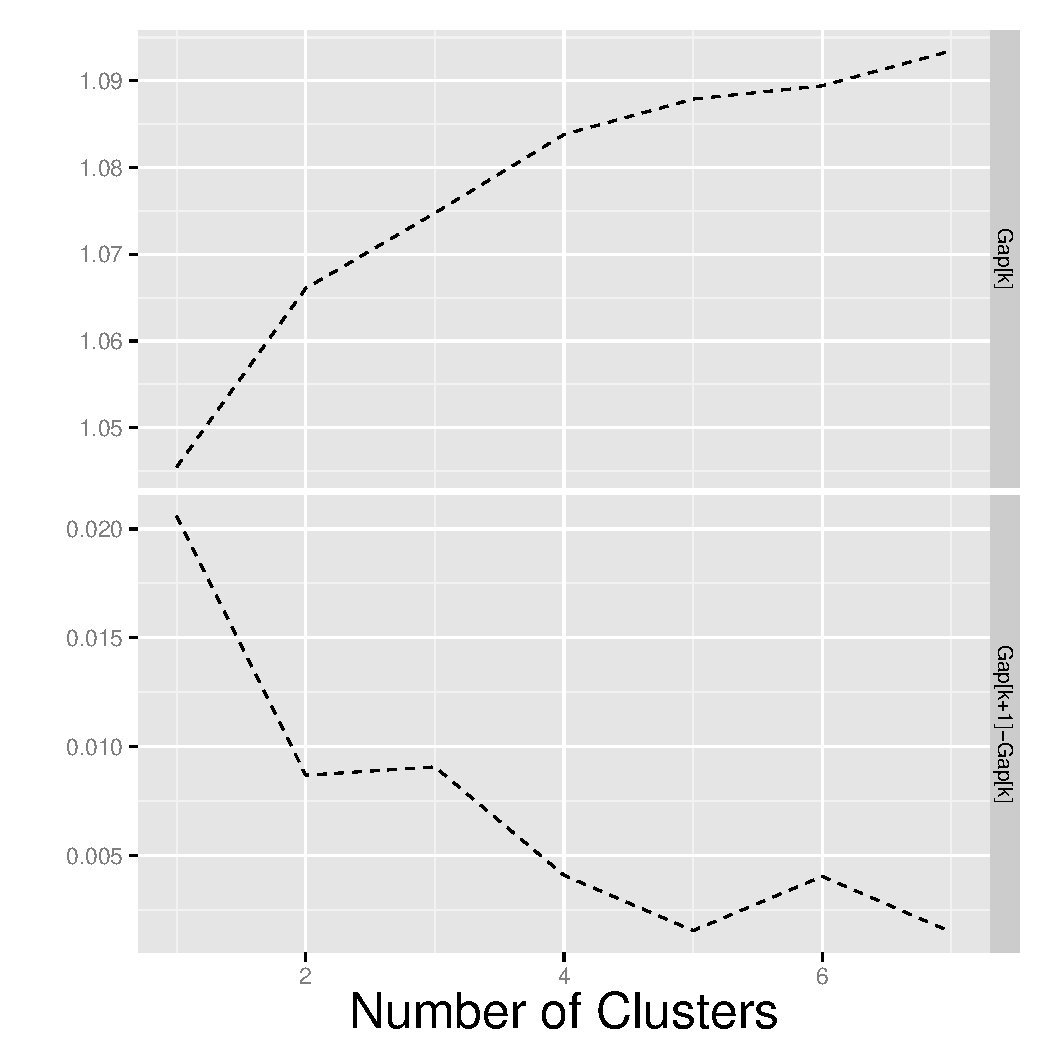
\includegraphics[width=\textwidth, height =0.8\textwidth]{fig/Gap_plot.pdf}
    \subcaption{}
  \end{minipage}
  \begin{minipage}[t]{0.33\textwidth}
    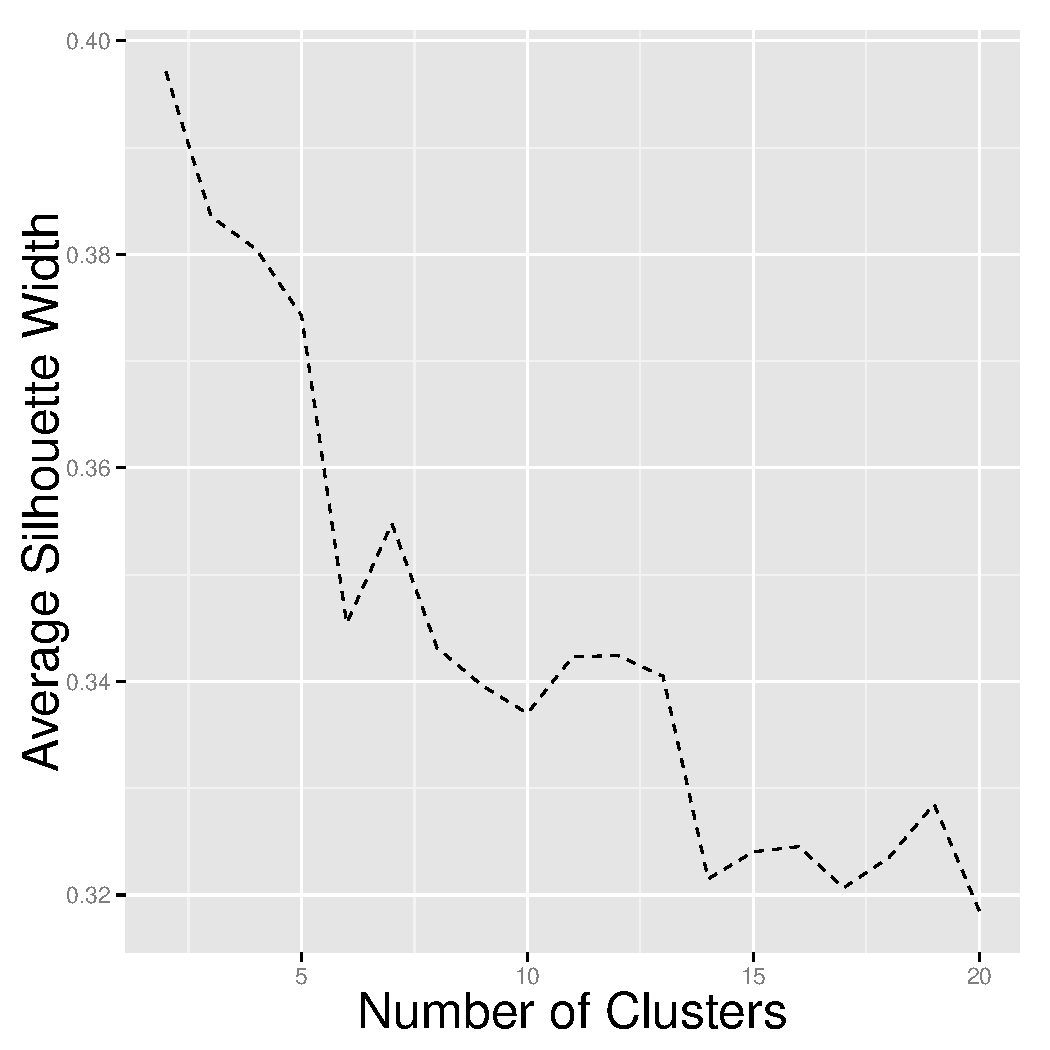
\includegraphics[width=\textwidth, height =0.8\textwidth]{fig/ave_sil.pdf}
    \subcaption{}
  \end{minipage}
  \begin{minipage}[t]{0.34\textwidth}
    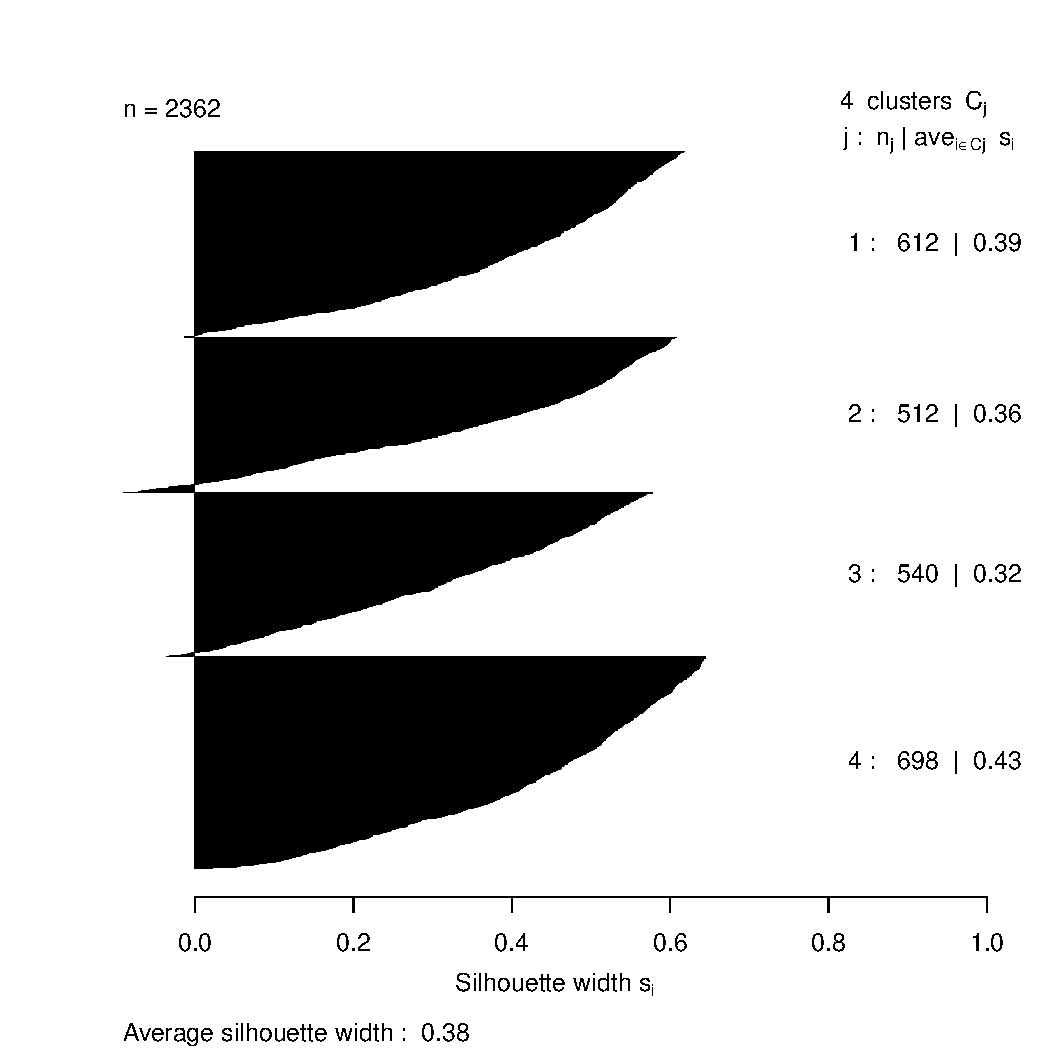
\includegraphics[width=1\textwidth, height =0.8\textwidth]{fig/sil_PCA_4.pdf}
    \subcaption{}
  \end{minipage}
  \caption{\textbf{Gap statistics and Silhouette plot for the number of clusters.} \textbf{(a)}Top: Gap statistics $Gap_k$; Bottom: The difference between consecutive Gap statistics $Gap_{k+1}-Gap_{k}$. \textbf{b} Average Silhouette width in terms of different numbers of clusters. \textbf{(c)} Silhouette plot when the number of clusters is 4.}
  \label{fig:Gap and Sil}
\end{figure*}


\qquad How to determine the number of clusters is the first concern before researches apply any kinds of clustering methods on their data. In our case, we solve the problem from both the qualitative and quantitative perspectives. The \textit{Gap} statistics \textbf([ref!]) \cite{gap} receives high popularity when it comes to \textit{k-means}. We calculate \textit{Gap} statistics for the number of clusters from 1 to 8 (See \textbf{Figure \ref{fig:Gap and Sil}(a)}). Instead of using the standard deviation of the simulated \textit{Gap} values because they are always lower than the corresponding difference, we determine to set the cutoff as 0.005. When the number of clusters goes to 4, the Gap statistics difference first falls below 0.005, hence we prefer to select 4 clusters. Furthermore, We take a look at the \textit{Silhouettes} plot \cite{silhouettes} of clustering with different numbers of clusters (See \textbf{Figure \ref{fig:Gap and Sil}(b)}). The average \textit{Silhouette} width for the number of clusters equal to 2, 3 and 4 all look good. However, combined with their associated \textit{Gap} statistics, the first two values are not preferred. Finally, the visualization also plays an important role in determining the cluster number. The rule is to find the number so that there are apparent geography groups while adding one cluster will lead to chaotic clustering (chaotic clustering means some groups distribute all over the country without obvious patterns) caused by overfitting. We compare the clustering maps with different numbers of clusters and find the map with four-clusters looks the most reasonable.\\


\qquad With slecting the cluster number as four, we apply k-means clustering on original data aggregated over county, as shown in
Figure~\ref{subfig:kmeansOnRawData}. In order to see the effectiveness 
of our data reduction, we apply k-means clustering on part of those
 principle components, i.e. the first 80, as shown in
Figure~\ref{subfig:kmeansOnReducedData}. As we can see from Figure~\ref{subfig:kmeansOnReducedData},
even only using the first 80 pcs, we can still produce a very good
cluster results, even a little bit smoother than raw data (since PCA can do denoising).\\

\qquad From the clustering results (Figure~\ref{subfig:kmeansOnRawData}), we can see \textit{New England} and \textit{Florida} belong to the red 
cluster. Many of the Northern dialects can trace their roots to this dialect which was spread westward by the New England 
settlers as they migrated west. It carries a high prestige due to Boston's early economic and cultural importance and the presence of Harvard University. 
In South Florida, there are those who consider that this region should be reclassified as part of the Northern dialect region. 
So many people from the North - particularly New York - have moved to south Florida that the majority of people tend to sound more Northern than Southern.
\textit{North Midland},
created as the people in Pennsylvania migrated westward and influenced by Scotch-Irish, German, and English Quaker settlers,  forms the central yellow cluster. The south part, is a continuous green continuum, including \textit{South Midland}, \textit{Virginia Piedmont}, 
\textit{Southern Appalachina}, and \textit{Gulf Southern}. South Midland, dominated by the Appalachian Mountains and the Ozark Mountains, was originally settled by the Pennsylvania Dutch moving south from the North Midland areas and the Scotch-Irish moving west from Virginia. In general south, as the northern dialects were originally dominated by Boston, the southern dialects were heavily influenced by Charleston, Richmond, and Savannah.
The rest of state, mainly the western regions, like \textit{Chicago Urban}, \textit{Upper Midwestern}, \textit{Rocky Mountain}, 
\textit{Pacific Northwest}, \textit{Southwestern}, and \textit{Pacific Southwest}, belong to the biggest blue continuum.
Compared with the Eastern United States, the Western regions were settled too recently for very distinctive dialects to have time to develop or to be studied in detail. Many words originally came from Spanish, cowboy jargon, and even some from the languages of the Native Americans.

\begin{figure}[t!]
    \centering
    \begin{subfigure}[t]{0.49\textwidth}
        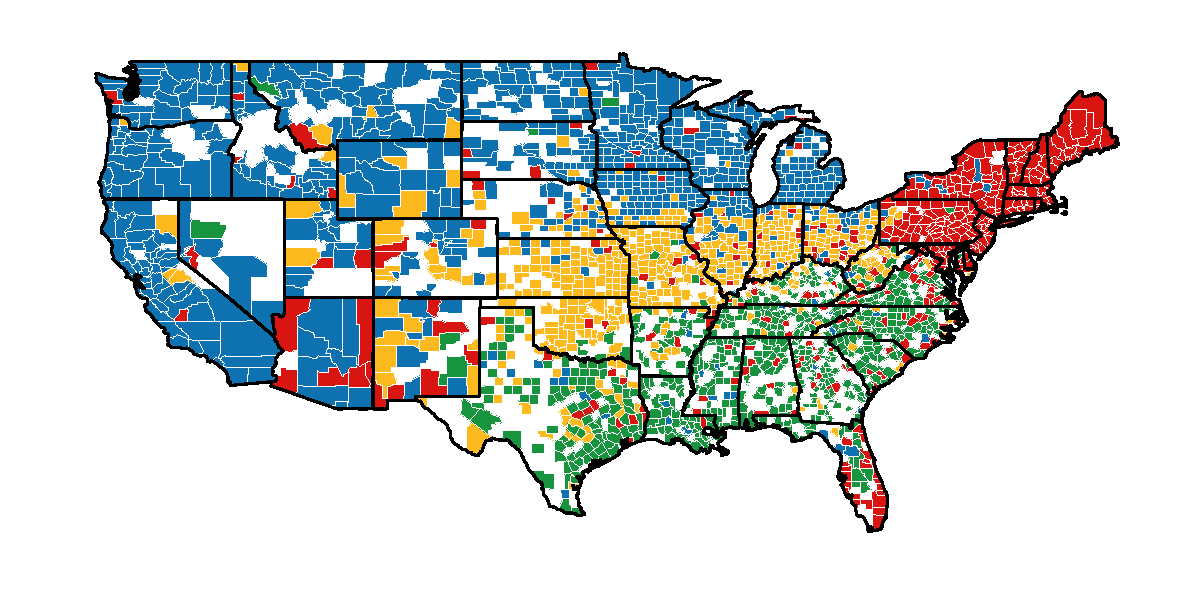
\includegraphics[width=1.1\textwidth]{fig/kmeans-original-data-4-cluster}
        \caption{raw data}\label{subfig:kmeansOnRawData}
    \end{subfigure}
    \begin{subfigure}[t]{0.49\textwidth}
        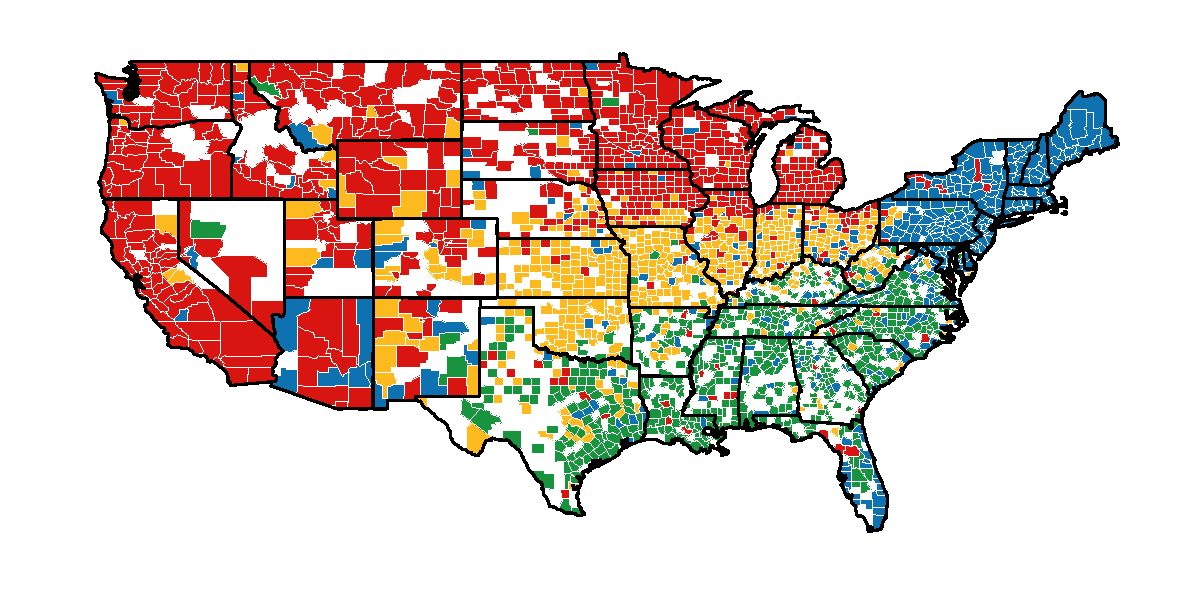
\includegraphics[width=1.1\textwidth]{fig/kmeans-reduced-data-4-cluster-80-pc}
        \caption{80 pcs}\label{subfig:kmeansOnReducedData}
    \end{subfigure}
    \caption{\textbf{The clustering map for kmeans on county level}
\textbf{(a)} raw data. \textbf{(b)} 80 pcs.}  \label{fig:kmeansClustering}
\end{figure}


\subsection{Non-negative Matrix Factorization (NMF)}

\qquad Non-negative matrix factorization, also non-negative matrix approximation is a group of 
algorithms in linear algebra where a matrix $V$ is factorized into two matrices $W$ and $H$, 
with the property that all matrices have no negative elements. NMF find applications in 
some fields as computer vision, document clustering, etc. NFM has the following form:

$$V = WH$$

\qquad It can be implemented as computing the columns vectors of $V$ as linear combination 
of the column vector of $W$ using coefficients supplied by columns of $H$.
In our case, matrix $V$ is the transpose of the original data matrix, in which each column
represents one data point (county level or person level). As NMF needs massive calculation, 
it is not realistic to do NMF on people level. Therefore, we apply NMF on the dataset 
aggregated by county.  We have done data reduction on the original dataset, i.e. PCA. 
However, here we are not able to apply NMF on reduced dataset, because NMF requires 
non-negative matrix.\\

\qquad One should realize that the results of NMF is not directly cluster ID. Instead, the 
results are coefficients of original data on the selected out ``bases''. In order to decide the 
cluster ID for each data point, here we simply choose the index of the maximal coefficient.\\

\qquad We tries $rank=3$ and $rank=4$ for NMF clustering, as shown
in Figure~\ref{fig:NMFClustering}. Comparing these plots, one can tell $rank=3$  is enough, 
because adding one more rank only bring us noises. 

\qquad It is worthy noting that, the results of NMF are essentially different from that of k-means. First, \textit{California}, \textit{Southwest} are now bunched with \textit{New England} and \textit{Florida} in the yellow cluster. This is also explainable. California actually combines elements of Western New England and Upper Midwestern. Especially, San Francisco continued to be settled by people from the Northeast and Northern Midwest, and elements of their dialects (North Midland, Upper Midwestern, Inland Northern) can be found. Mission dialect, spoken by Irish Catholics in a specific part of the city is very much like the New York City dialect. Second, \textit{Michigan} now is also in the same cluster with \textit{New England}, since the \textit{Upper Midwestern} is originally settled by people from New England and New York State who brought those dialects. Third, no matter we choose $rank=3$ or $rank=4$, the \textit{North Midland} and \textit{Upperwest} are no longer separable as in the results of k-means clustering, which is not quite explainable from a linguistic perspective. 



\begin{figure}[t!]
    \centering
    \begin{subfigure}[t]{0.49\textwidth}
        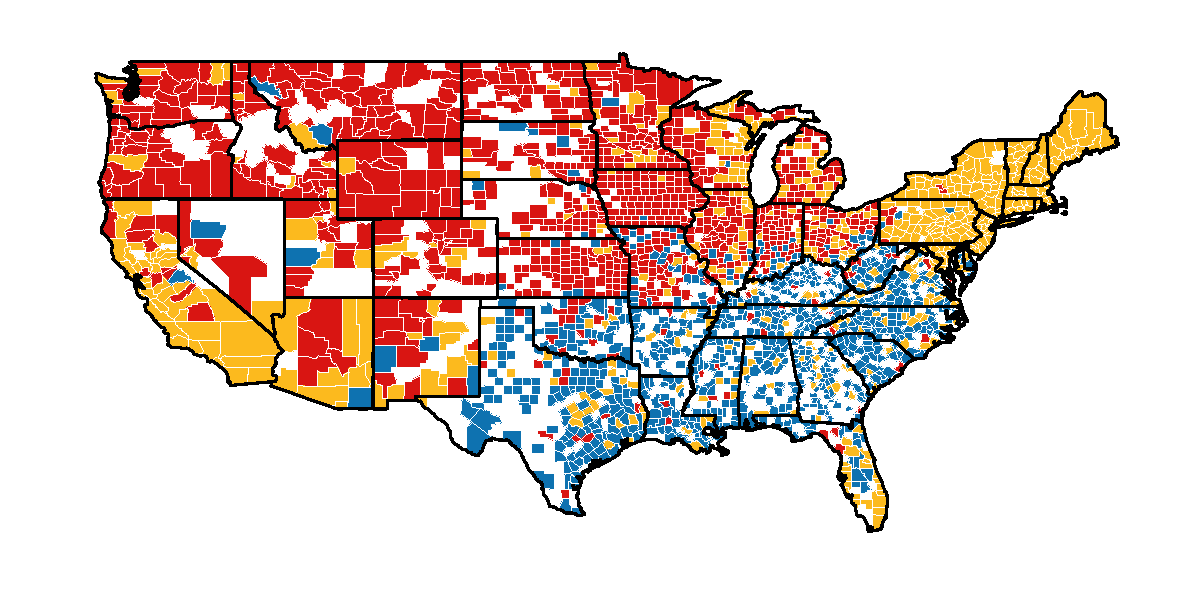
\includegraphics[width=1.1\textwidth]{fig/nmf-original-data-3cluster}
        \caption{3 clusters}\label{subfig:NMFClustering3Clusters}
    \end{subfigure}
    \begin{subfigure}[t]{0.49\textwidth}
        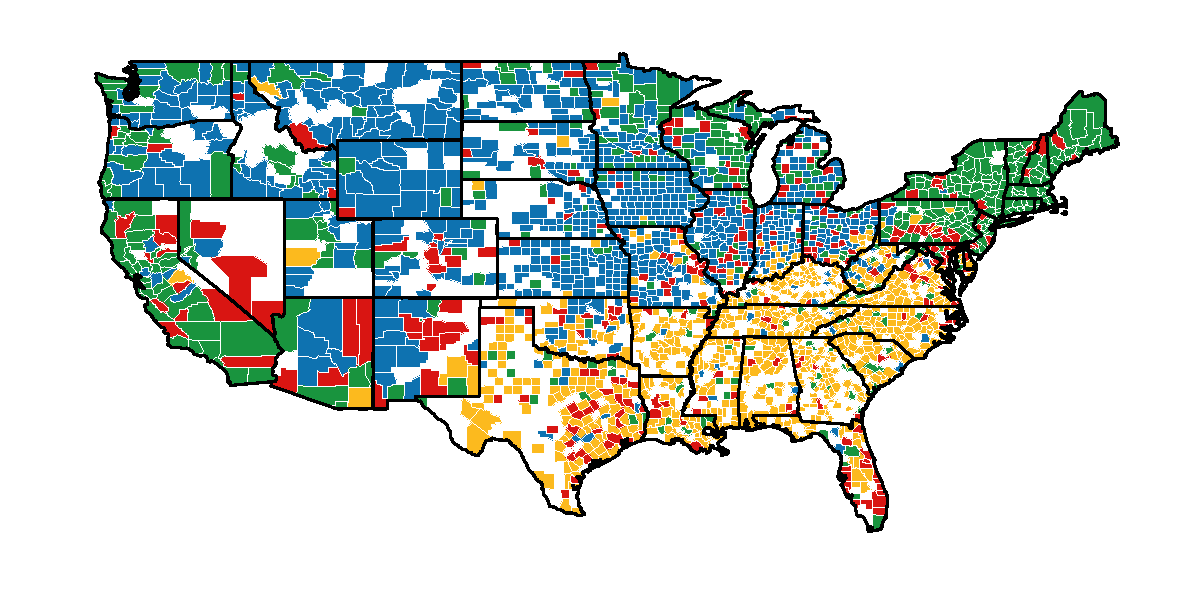
\includegraphics[width=1.1\textwidth]{fig/nmf-original-data-4cluster}
        \caption{4 clusters}\label{subfig:NMFClustering4Clusters}
    \end{subfigure}
    \caption{\textbf{The clustering map for NMF on county level}
\textbf{(a)} $k=3$. \textbf{(b)} $k=4$.}  \label{fig:NMFClustering}
\end{figure}
\subsection{k-medoids clustering}

\qquad The \textit{k-medoids} clustering method is similar to \textit{k-means}, except that the former takes $k$ data points as centers while the latter makes use of means from $k$ disjoint sets. The \textit{k-medoids} algorithm first picks up k data points randomly, and assign other points to their nearest centers, thus forming k clusters. Within each cluster, select the data point which minimizes the sum of the distances  between it and other points. Repeat the previous steps until convergence. Our \textit{k-medoids} clustering is based on the data of county level because for individual level there will be too many samples for the algorithm to work. Instead of using \textit{Gap} statistics and \textit{Silhouette} plot, this we mainly rely on visualization to determine the number of clusters because both the former methods tend to be conservative \textbf{[ref!]} and the performance looks very good when the cluster number is big. We finally determine to use six clusters after compare many of a great many scenarios (See  \textbf{Figure \ref{fig: k-medoids_reference}(b)} and see \href{https://yeyt2718.shinyapps.io/map_Question}{Map Set} for more).

\qquad We test the performance of \textit{k-medoids} on dialect clustering and compare the power between with and without data reduction. Apart from checking the clustering from raw data, \textit{PCA}, \textit{ICA} and \textit{Random Projection} are used to reduce the data dimension and eliminate noise within the data (See \href{https://yeyt2718.shinyapps.io/map_Question}{Map Set}). A tradeoff should be taken about taking how many components since too few components will lead to the loss of information. A thumb of rule is using visualization to help decide the number of components we are supposed to take. For example, we extract the top 80 principal components for further clustering after comparing the performance within the top 40, 60, 80, 100, 200, 300 components. Such data reduction makes the clustering much better than from the raw data. In \textbf{Figure \ref{fig: k-medoids_reference}(a)}, i.e., the clustering map for the raw data, there are four apparent dialects geography and continuum. But the blue and green regions scatter around. It is hard to tell the medoids  of the yellow, blue and green regions. In \textbf{Figure \ref{fig: k-medoids_reference}(b)}, i.e., the clustering map for 80 PCs, all the clustering regions display well-distributed. It's very easy to distinguish the medoids for each regions and each region is a continuum.


\qquad  Comparing \textbf{Figure \ref{fig: k-medoids_reference}(b)} and \textbf{Figure \ref{fig: k-medoids_reference}(c)}, we find that our clustering results based on 6 clusters with top 80 PCs are quite satisfactory. The violet region in \textbf{(b)} aggregate \textit{Rockey Mountain, Pacific Northwest, Pacific Southwest} in \textbf{(c)}. These Western regions were settled to recently for obviously distinctive dialects to have time to develop. Western people's words originate from Spanish, cowboy jargon and some Native Americans. The brown region in \textbf{(b)} corresponds to \textit{Upper Midwestern, Chicago Urban} in \textbf{(c)}. \textit{Upper Midwestern} were settled by people from \textit{New England} and \textit{New York State} with their dialects. This area was also influenced by Southerners coming up the Mississippi River as well as the speech patterns of the German and Scandinavian immigrants and the Canadian English dialects from over the border. The blue region in \textbf{(b)} corresponds to \textit{New England, Inland Northern} in \textbf{(c)}. This area is the very earliest settlement from Europe and many of the Northern dialects can trace their roots to this dialect wihch was spread westward by the \textit{New England} as they migrated west. The red region in \textbf{(b)} corresponds to \textit{North Midland} in \textbf{(c)}. This area was created as the people in Pennsylvania migrated westward and influenced by Scotch-Irish, German, and English Quaker settlers. The yellow region in \textbf{(b)} corresponds to the main part of\textit{ South Midland, Southern Appalachian, Coastal Southern} in \textbf{(c)}. The southern dialects were heavily influenced by Charleston, Richmond, and Savannah. But notice that \textit{South Florida} should be reclassified as part of the Northern dialect region. So many people from the North - particularly New York - have moved here that the majority of people tend to sound more Northern than Southern. The green region in \textbf{(b)} corresponds to the main part of \textit{Southwestern, GulSouthern} in \textbf{(c)}. The Mexican dialect of Spanish had an significant influence on this area because there had already been as many as ten generations of Spanish speakers live there by the time \textit{Southwestern} became part of the United States (Refer to \href{http://robertspage.com/dialects.html}{Dialect Map of American English} for more details).

\begin{figure}[t!]
    \centering
    \begin{subfigure}[t]{0.49\textwidth}
        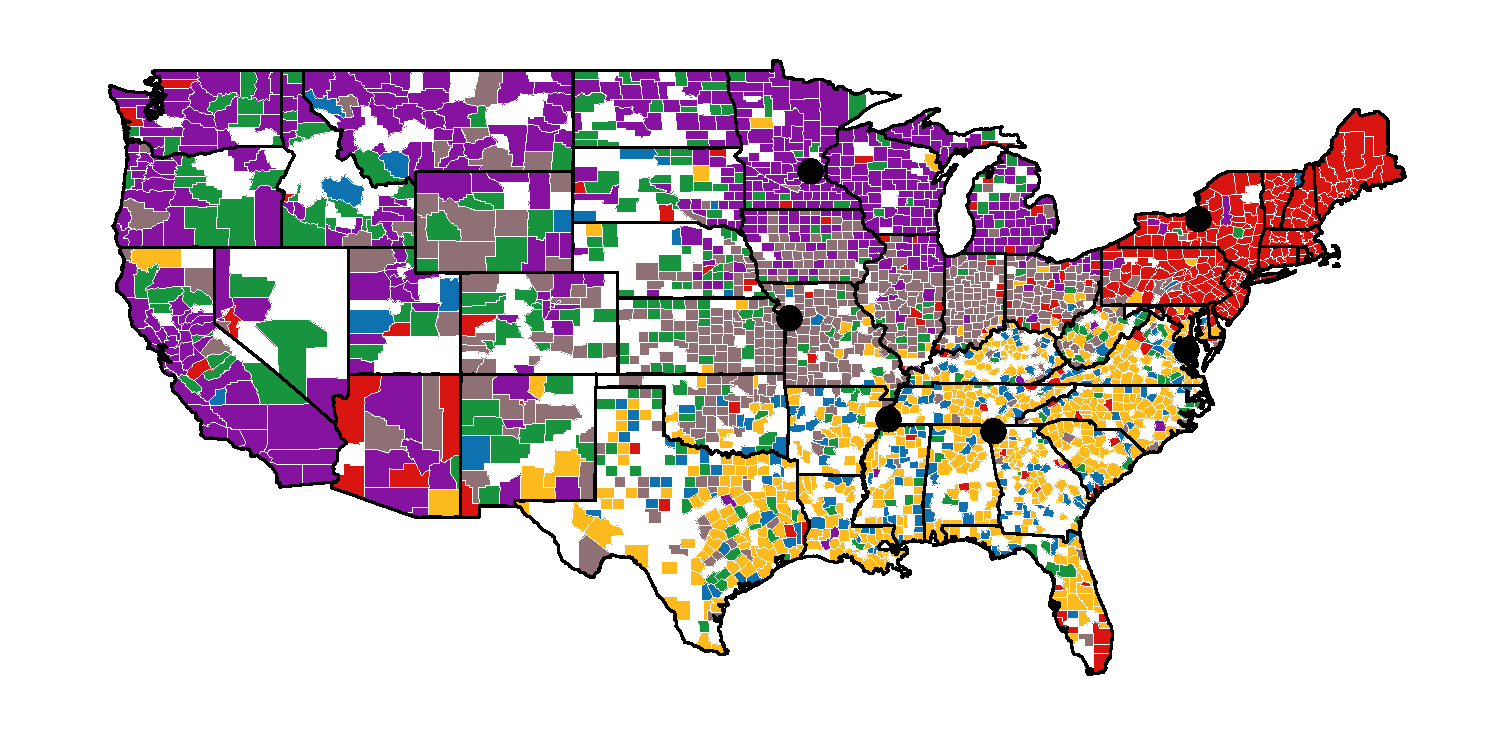
\includegraphics[width=1\textwidth]{fig/kmedoids6_raw.pdf}
        \caption{raw data with 6 clusters}
    \end{subfigure}
    \begin{subfigure}[t]{0.49\textwidth}
        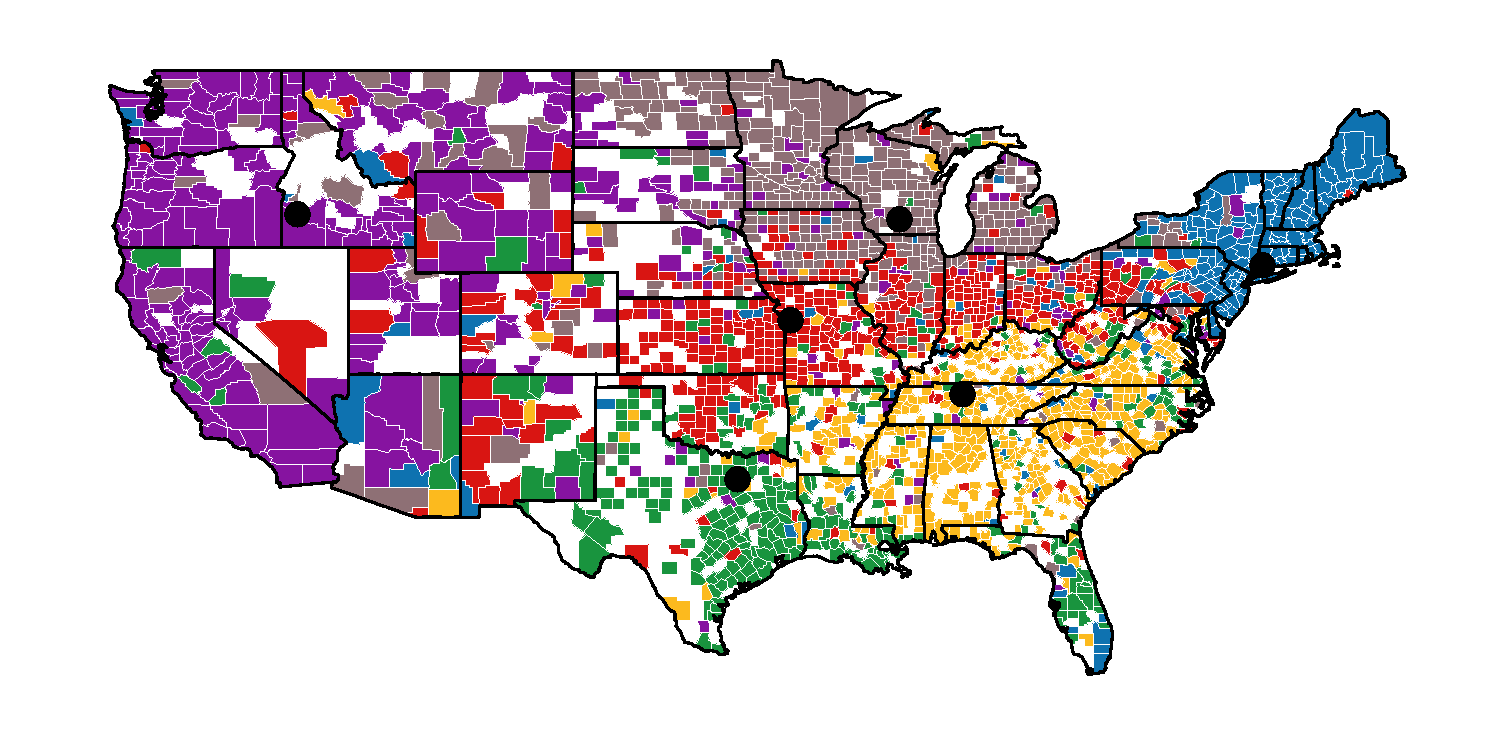
\includegraphics[width=1\textwidth]{fig/kmedoids6_PCA80.pdf}
                \caption{top 80 PCs with 6 clusters}
    \end{subfigure}
        \begin{subfigure}[t]{\textwidth}
        \centering
        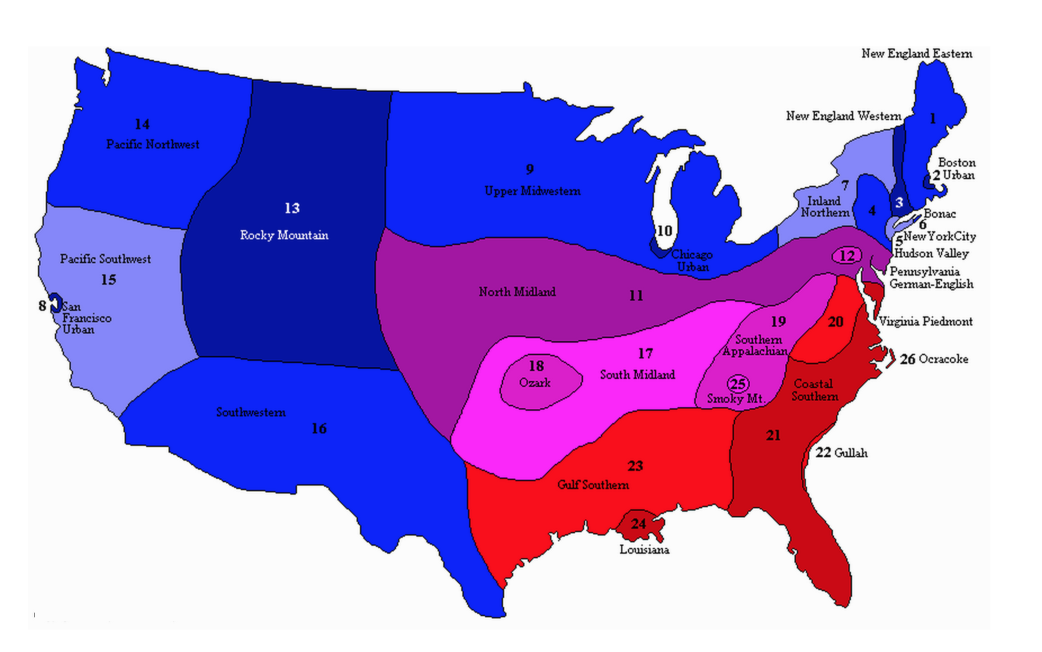
\includegraphics[width=0.6\textwidth, height= 0.4\textwidth]{fig/reference_map.pdf}
                \caption{Dialect Map of American English}
    \end{subfigure}
    \caption{\textbf{The clustering map for k-medoids when $k = 6$ on county level.} \textbf{(a)} Clustering based on the raw data with 6 clusters. \textbf{(b)}  Clustering based on the top 80 PCs with 6 clusters. The four black points are medoids. \textbf{(c)} \href{http://robertspage.com/dialects.html}{Dialect Map of American English} .} \label{fig: k-medoids_reference}
\end{figure}

\subsection{Hierarchical Clustering}
\begin{figure}
  \begin{minipage}[b]{0.5\columnwidth}
    \centering
    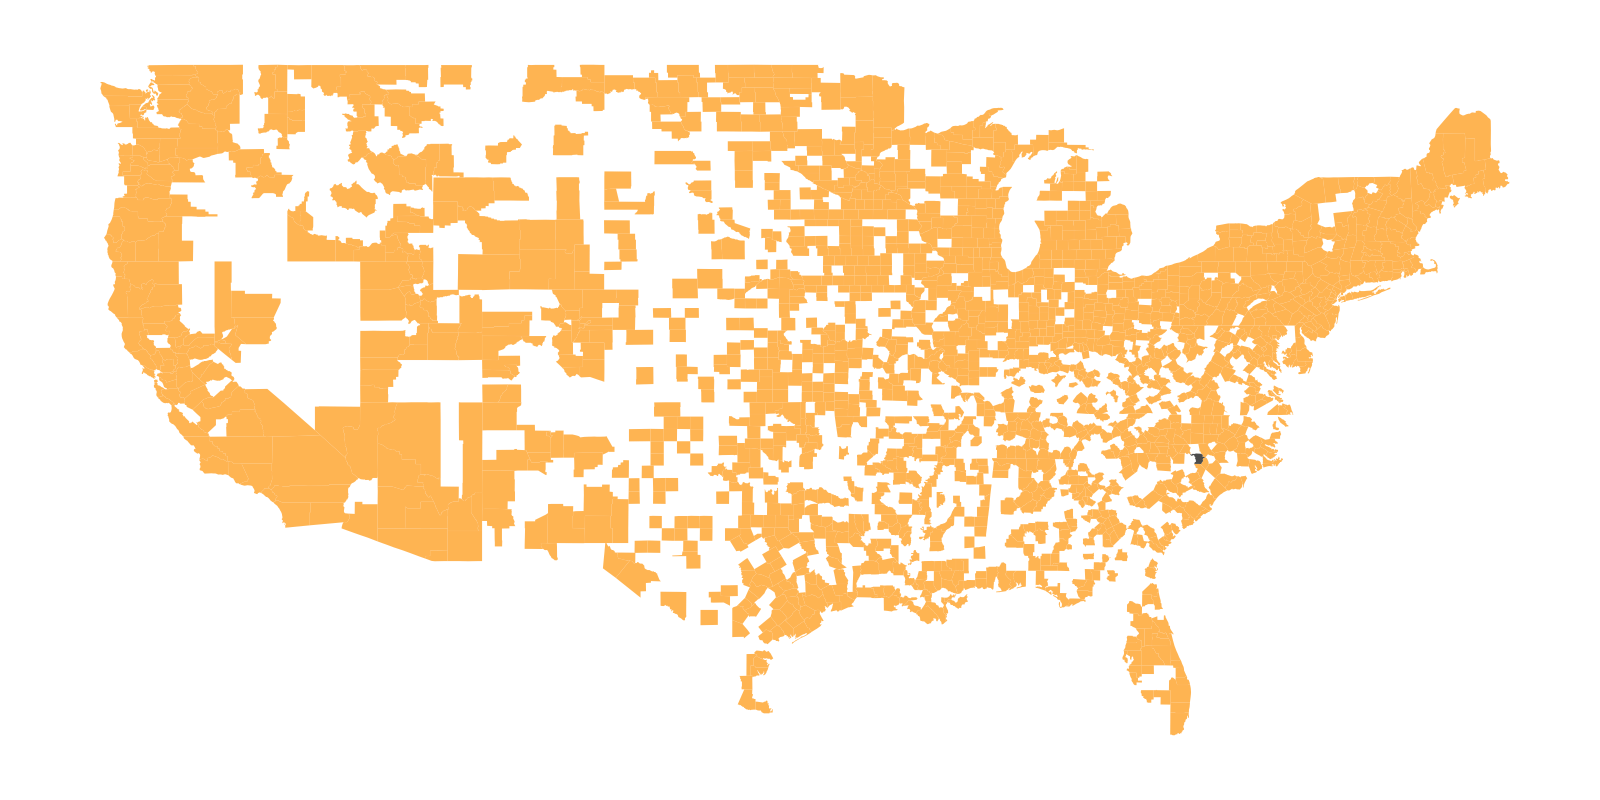
\includegraphics[width=\columnwidth]{fig/hierarchical1.png}
    \subcaption{Depth=1}\label{subfig:hierarchy1}   
  \end{minipage}
  \begin{minipage}[b]{0.5\columnwidth}
    \centering
    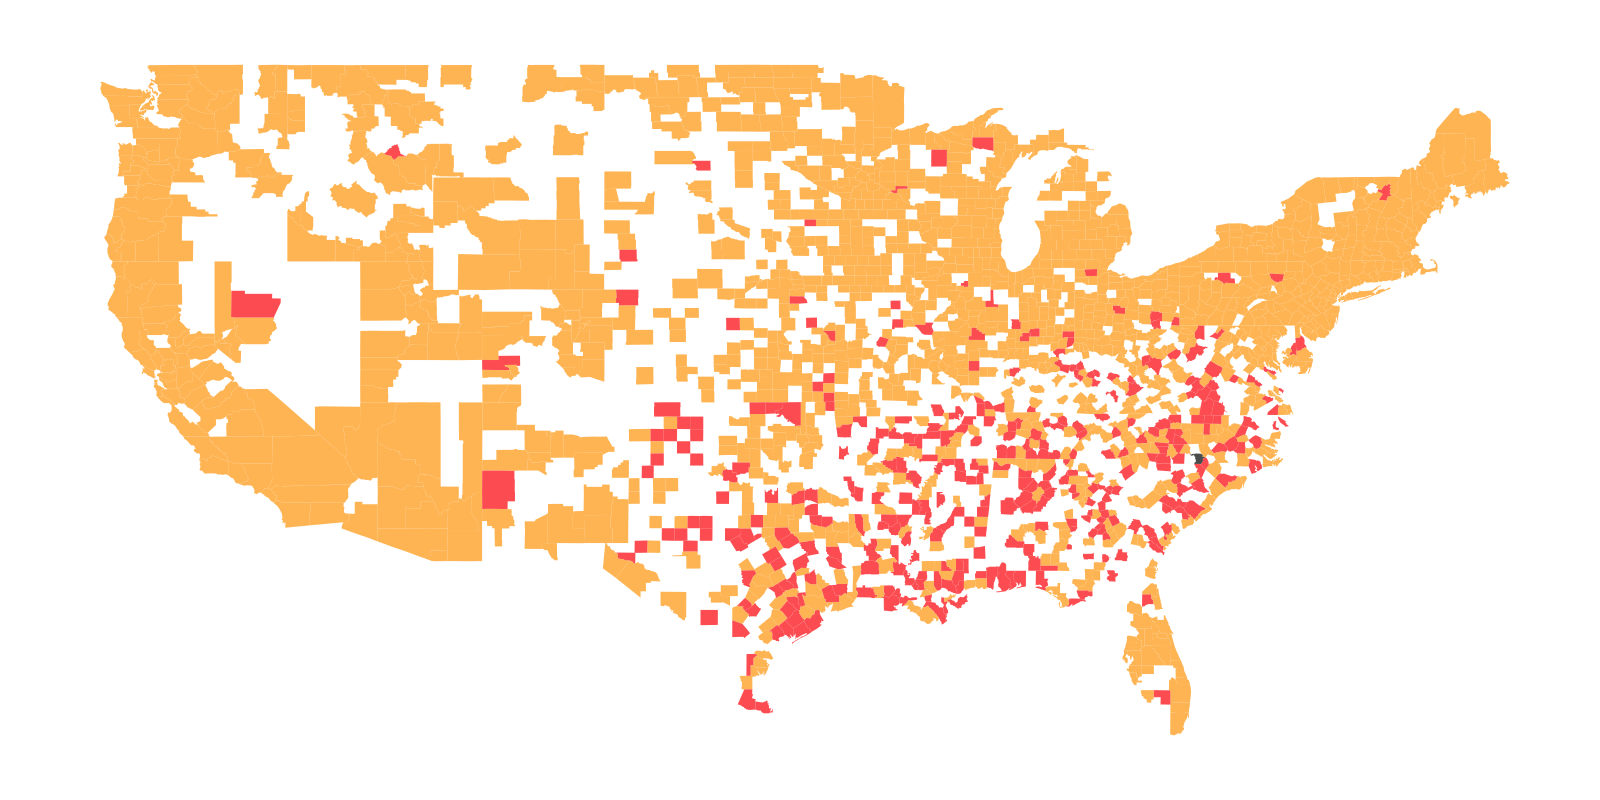
\includegraphics[width=\columnwidth]{fig/hierarchical2.png}
    \subcaption{Depth=2}\label{subfig:hierarchy2}
  \end{minipage}\\
  \begin{minipage}[b]{0.5\columnwidth}
    \centering
    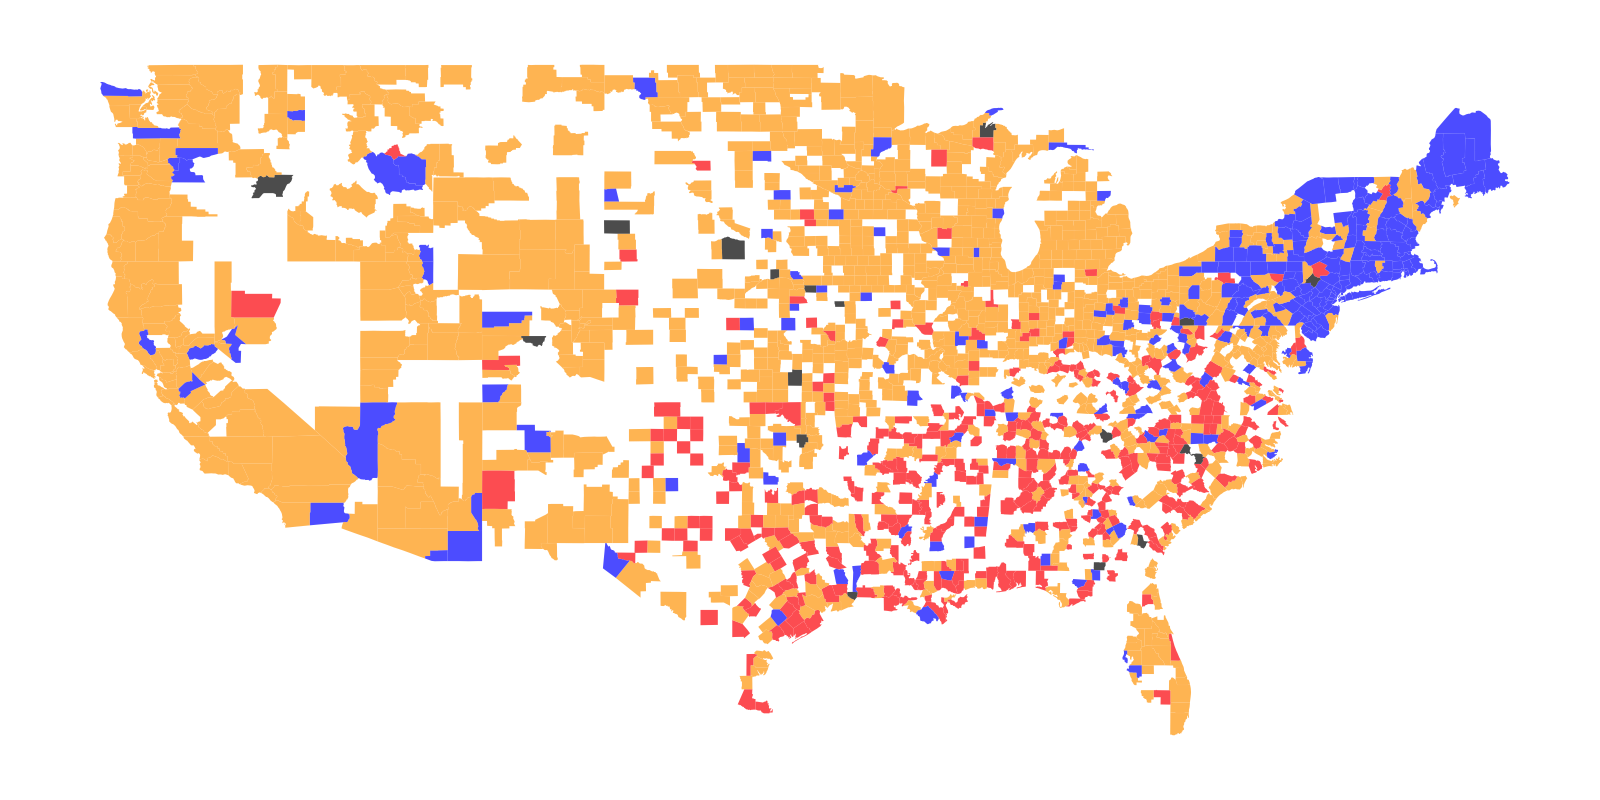
\includegraphics[width=\columnwidth]{fig/hierarchical3.png}
    \subcaption{Depth=3}\label{subfig:hierarchy3}
  \end{minipage}
  \begin{minipage}[b]{0.5\columnwidth}
    \centering
    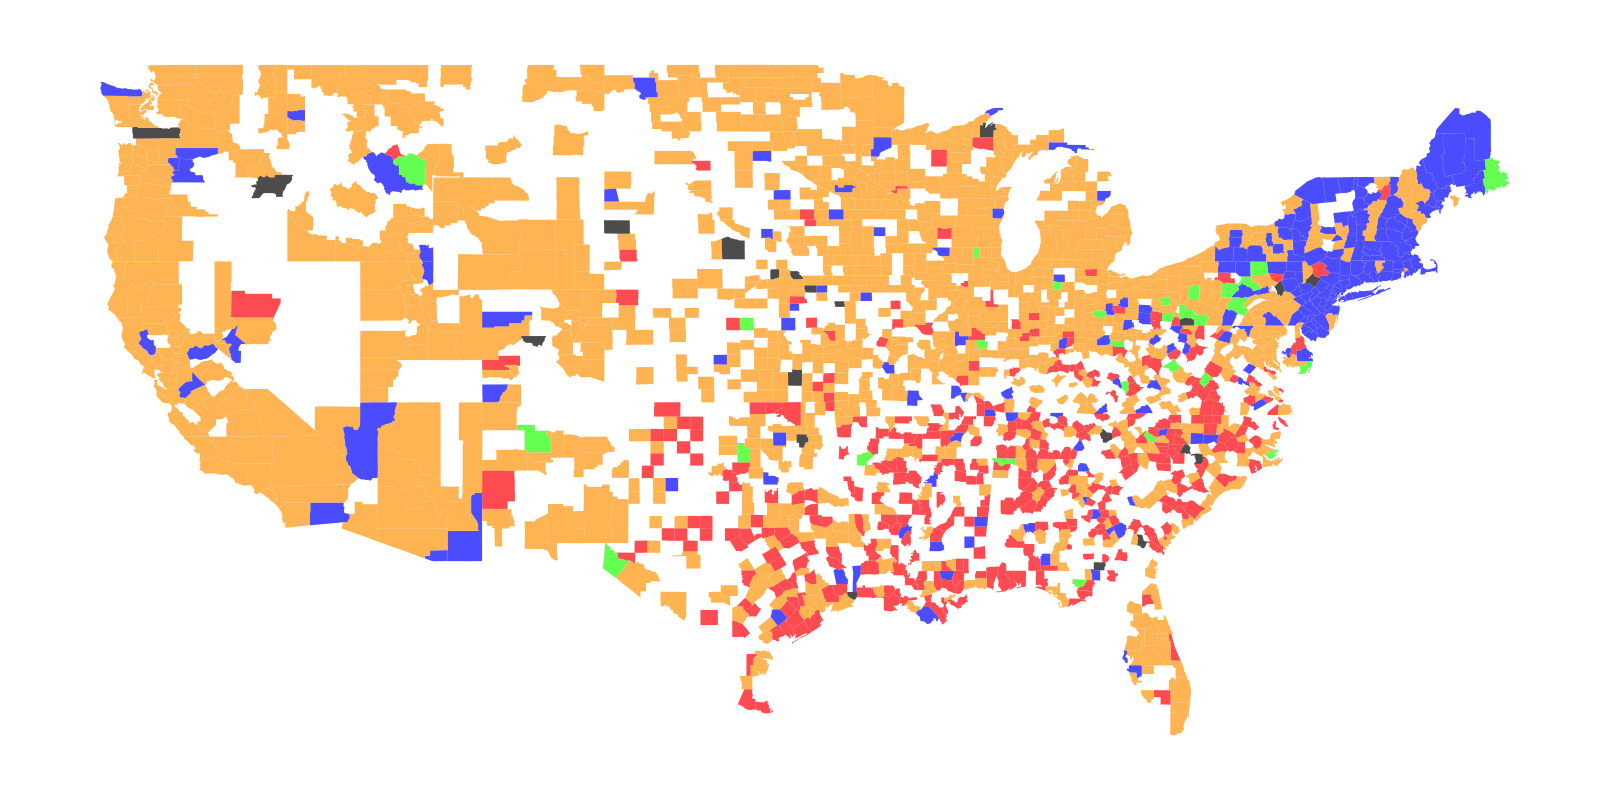
\includegraphics[width=\columnwidth]{fig/hierarchical4.png}
    \subcaption{Depth=4}\label{subfig:hierarchy4}
  \end{minipage}\\
  \begin{minipage}[b]{0.5\columnwidth}
    \centering
    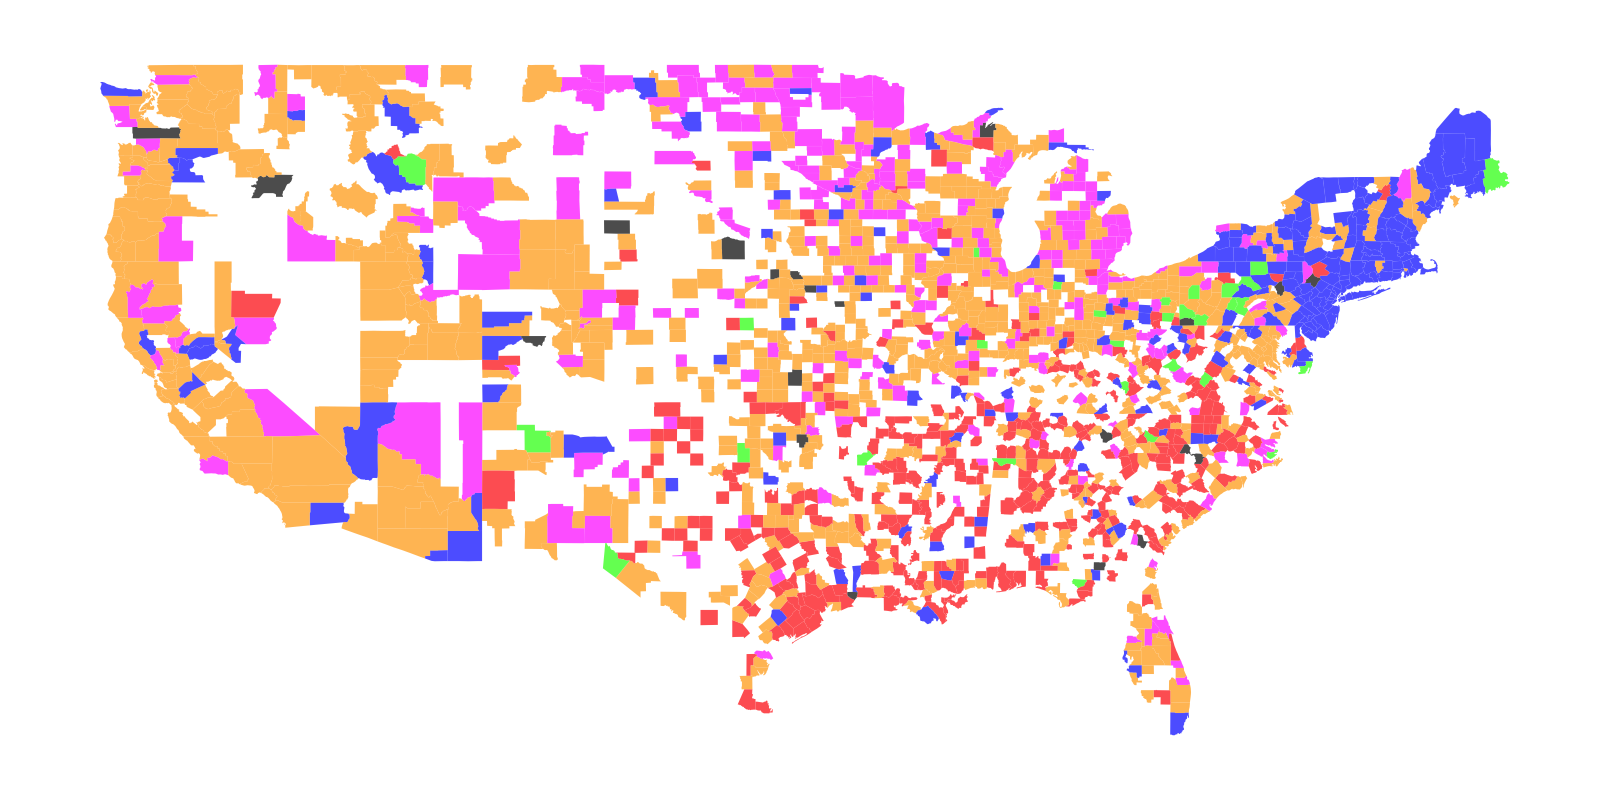
\includegraphics[width=\columnwidth]{fig/hierarchical5.png}
    \subcaption{Depth=5}\label{subfig:hierarchy5}
  \end{minipage}
  \begin{minipage}[b]{0.5\columnwidth}
    \centering
    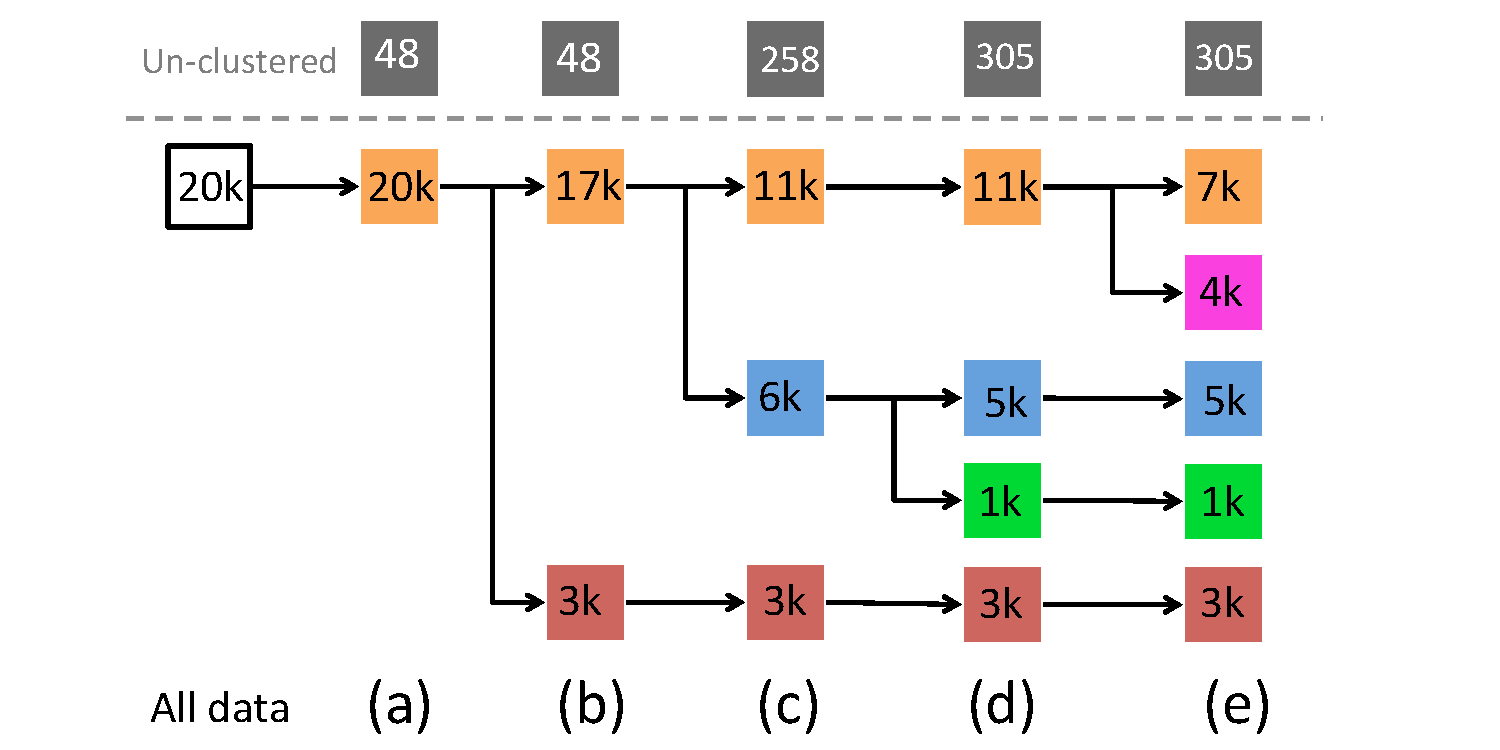
\includegraphics[width=\columnwidth,height=0.4\columnwidth]{fig/hierarchy.pdf}
    \subcaption{The hierarchy.}\label{subfig:hierarchy}
  \end{minipage}\\
  \caption{Hierarchical clustering. (a)-(e) gives clustering map at different hierarchy depth. (f) shows the hierarchy and number of observations that fall into each cluster.}
  \label{fig:hierarchy}
\end{figure}

\qquad  {\it Hierarchical clustering} is another method for clustering which finds a hierarchy of clusters. The result of hierarchical clustering can be presented as a dendrogram, a tree-like structure with a depth of $n-1$, where $n$ is the number of observations. At each depth, the dendrogram specifies which cluster can be further splitted into two small clusters, thus constructing the hierarchy. 

\qquad  By applying hierarchical clustering to our dialet dataset, we seek to find possible hierarchies in dialect regions. In other words, are there dialect regions that are closer to each other? Which dialect region has the most dissimilar language?

\qquad  When we apply hierarchical clustering to the datast, we find the following decisions to be relevant:

\begin{itemize}
\item \textbf{Sampling} We soon realize that we have to sample the dataset for faster processing. Hierarchical cluster requires pre-computing a pair-wise dissimilarity matrix between all observations. With 43265 observations, and 4 bytes per dissimilarity value in R, storing the matrix requires 6.97 GB of memory. This is beyond the memory capacity of any single machine we have. One way to reduce memory footprint is to trade off computation speed by creating dissimilarity values only when needed. For example, with {\it fastcluster::hclust.vector}, we don't need to create the matrix and finish one run of clustering with $\sim$67 minutes. We eventually decided to down-sample the data by half so that we could fit the entire dissimilarity matrix (1.6GB) in memory. This allows us to perform fast ($\sim$15s/run) clustering with various settings. We find that half sampling has limited impact on the findings we reach.

\item \textbf{Clustering Type} There are two types of hierarchical clustering: \textbf{Agglomerative} and \textbf{Divisive}, differentiated by how the computation starts. \textbf{Agglomerative} starts with each observation as a single cluster, and merge pairs of clusters until only one cluster is left. \textbf{Divisive} starts with a single cluster with all observations, and split clusters recursively until each observation has its own cluster. We choose \textbf{Agglomerative} due to lack of efficient \textbf{Divisive} implementations. 

\item \textbf{Dissimilarity Metric} determines how distance between two observations is calculated. We choose ``Manhattan distance'', which effectively captures how many questions a pair of participants have different answers (scaled by 2).

\item \textbf{Linkage Metric} determines how distance between two clusters are computed. We tried ``Single''(nearest neighbor method), ``Average'', ``Complete''(furthest neighbor method), ``Median'', ``Centroid'' and ``Ward''(minimizing within-cluster sum of squares). While most of the metrics lead to clusters of extreme size difference, we find ``Complete'' and ``Ward'' to be useful for generating clusters with similar diameters. 
\end{itemize}

\qquad  Figure~\ref{subfig:hierarchy} shows the hierarchy of first five depths when using the ``Complete'' metric. Each color box represents a cluster separated at that depth, with the number of samples in that cluster. Moving down the hierarchy, at each depth, one cluster is split into two small clusters at the next depth. This means that 1) the two small clusters are the closest pair at their depth; 2) the two small clusters are the furthest pair at one depth lower. 

\qquad  With the above observations, let's look at Figure~\ref{subfig:hierarchy1}$\sim$\ref{subfig:hierarchy5}, where we show the clusters on the geographic map. The first thing we notice is that the {\em Southern} dialect region is the first region to be identified, as shown in Figure~\ref{subfig:hierarchy2}. This means that the {\em Southern} region is most different compared to the rest of the country. With ``Ward'' as the linkage metric, the first identified region is the {\em New England East} region in northeast, which happens to be the second identified region under ``Complete'', as shown in Figure~\ref{subfig:hierarchy3}. Going downward the hierarchy, it is less clear that which specific region is identified, although clustering effect could still be observed. Compare the eventual separation in Figure~\ref{subfig:hierarchy5}, we find that clustering is noisier compared to k-means. We attribute this to the non-iterative nature (a observation will not be moved out of a cluster) of hierarchical clustering, as well as the fact that both linkage metrics we use, ``Complete'' and ``Ward'', are not robust to outliers.

\qquad  An animated version of the clustering results can be accessed at \url{https://goo.gl/photos/7udEt9JFmDVjw7676}.
\subsection{Comparing Clustering Results: Hungarian Algorithm}

Since we tried different clustering methods, it would be vital to come
up with a statistics to compare different clustering
results. Essentially, there should be two steps in this procedure. \\

\noindent Let say we are going to compare two clustering results, $C$
and $C^{'}$, each containing $n$ clusters, i.e. $c_1, c_2, ... c_n$
and $c^{'}_1, c^{'}_2, ... c^{'}_n$.\\

\noindent First step is to determine an one to one mapping
$$f: \{c_i: i=1...n\} \rightarrow \{c^{'}_i: i=1...n\}$$

\noindent Given a mapping $f$, we can compute the Rand Index for the
two clustering results, which is a typical measure of the similarity
between two data clusterings.\\

\noindent We are supposed to find a mapping $f$ to maximize the
similarity (Rand Index), and take the maximal Rand Index as a
similarity measure of the two clustering results, as described by
Hungarian Algorithm\cite{hungarian} (The Hungarian method is a combinatorial
optimization algorithm that solves the assignment problem in
polynomial time and which anticipated later primal-dual methods. It
was developed and published in 1955 by Harold Kuhn, who gave the name
``Hungarian method'' because the algorithm was largely based on the
earlier works of two Hungarian mathematicians).


\subsection{Finding Critical Questions dominating clustering Results}

Here we intend to figure out which of those questions are most
critical forclustering. To be consistent, here we always perform k-means
clustering on original data aggregated over county. We set the k-means
results of the whole dataset as ``standard clustering''.\\

\noindent To see how important a question is, we remove the
corresponding column for that question from the original dataset, and
then apply k-means clustering on the new dataset. After that, using
the method mentioned previously, we compute a similarity measure
between this clustering results and the ``standard clustering''. We
perform this procedure ten times on each of the 67 questions and take the average similarity measure (k-means is not perfectly stable), as shown in
Figure~\ref{fig:removeQuestion}.\\


\begin{figure}
\centering
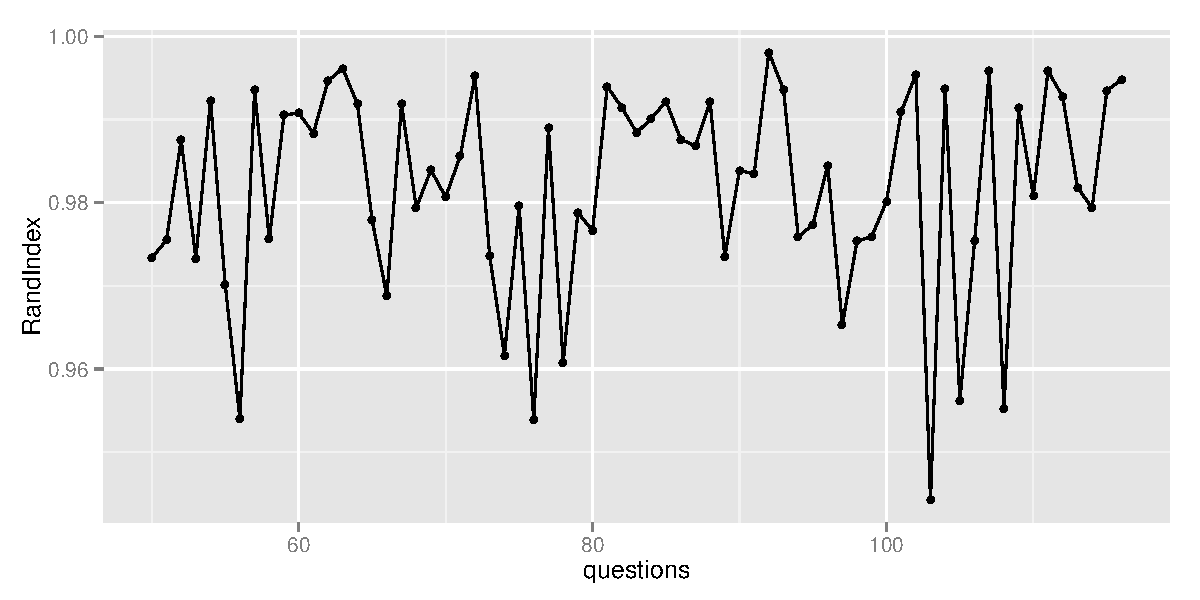
\includegraphics[width=0.9\linewidth]{fig/remove-question-clustering-difference.pdf}
\caption{remove-question-clustering-difference} \label{fig:removeQuestion}
\end{figure}

\noindent As we can see from Figure xx, clearly there are 5 questions
perturbing the clustering results significantly, which are question
56, 76, 103, 105, 108. From the Dialect Survey website, we have these
four questions as follow:

\begin{itemize}

\item Q056: Pantyhose are so expensive anymore that I just try to get
a good suntan and forget about it.

\item Q076: What term do you use to refer to something that is across
both streets from you at an intersection (or diagonally across from
you in general)?

\item Q103: What do you call the thing from which you might drink
water in a school?

\item Q105: What is your generic term for a sweetened carbonated
beverage?

\item Q108: What vowel do you use in bag?


\end{itemize}

\noindent We are lucky to pick out Q076 in section 2 by visually
selection. The plots for the answer of each of these four questions
can be found in our \textbf{Shiny} app.


%\section{Stability of findings to perturbation}
\section{Stability of findings to perturbation}
\label{sec:stability}

\qquad Among all the clustering methods, we notice that \textit{k-means} clustering performs very well and data reduction methods like PCA are not able to improve it. Hence, we use \textit{k-means} to test the stability of the clustering results, based on county-level raw data. Several ways are proposed to perturb the data, i.e., adding noises, removing some columns (excluding some questions) or removing some surveyed people. Since we have got the conclusion that different questions possess distinct weights on determining separate groups or determining the continuum, it's not appropriate to sample questions for testing.  Besides, question design is the very thing researchers can control, so there is no need to check the influence of the missing questions. Moreover, excluding some individuals who took part in the survey is equivalent to adding noises to the data. We only consider adding some gaussian noises on the data columns and the data rows respectively. To see how robust \textit{k-means} is,  different levels of gaussian noises are added to the data. We generate noises of levels $0.05, 0.1, 0.15, 0.2, 0.25, 0.3$, each level with 10 replicates. Here, the noise of level $0.1$ means it comes from the gaussian distribution with mean of zero and standard deviation of  the sample mean multiplied by $0.1$. 

\qquad  We first check the influence of different \textit{k-means} starting points by setting several seeds. All their associated clustering maps look almost the same as \textbf{Figure xxx}, which implies \textit{k-means} always leads to the same clustering at least for the dialect problem. Furthermore, the \textit{Rand Index} is calculated between the clustering from noised data and that from the raw data to evaluate the robustness. The \textit{k-means} clustering performs quite robustly with different levels of noises (See \textbf{Figure \ref{fig:perturbation}(a)(b)}). When the noise becomes stronger, the corresponding clustering goes farther from the standard one as expected. But the \textit{Rand Index} is always higher than 0.94. Slight difference is observed when adding noises to data rows and data columns respectively, except that clusterings for the latter situation have higher variances (See \textbf{Figure \ref{fig:perturbation}(c)}). Such phenomenon indicates that changing questions may lay more influence on the results than changing surveyed subjects.

\begin{figure*}
  \begin{minipage}[t]{0.33\textwidth}
    \centering
    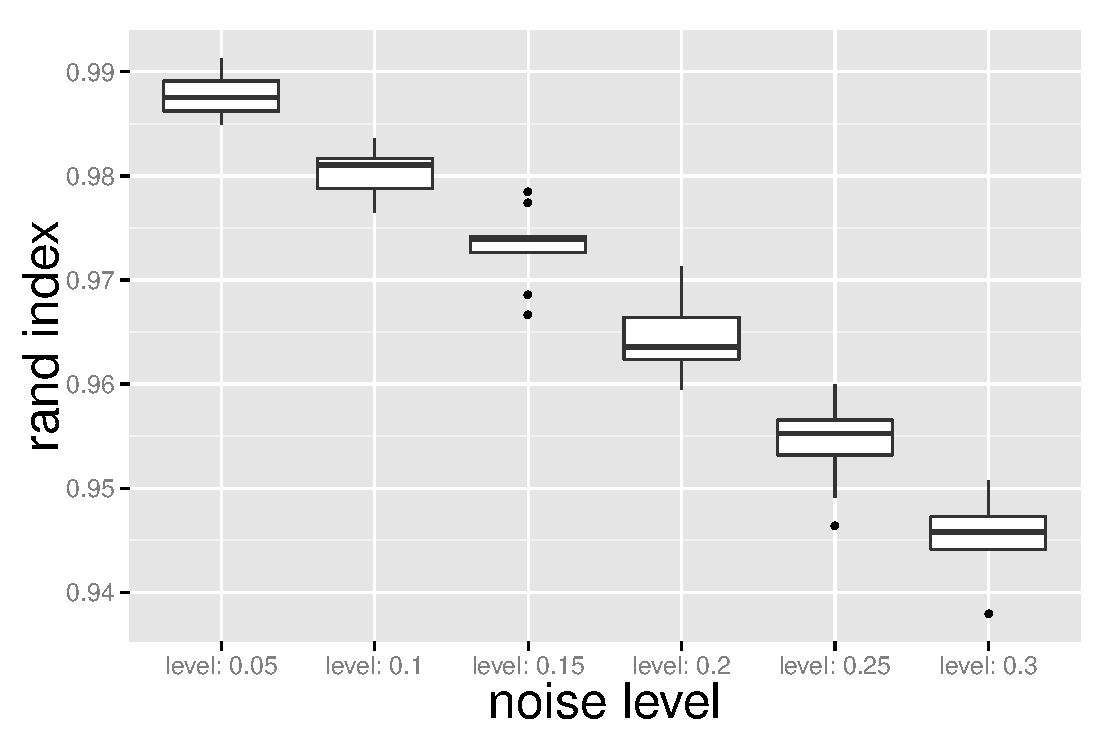
\includegraphics[width=\textwidth,height=0.8\textwidth]{fig/noise_boxplot_row.pdf}
    \subcaption{}
  \end{minipage}
  \begin{minipage}[t]{0.33\textwidth}
    \centering
    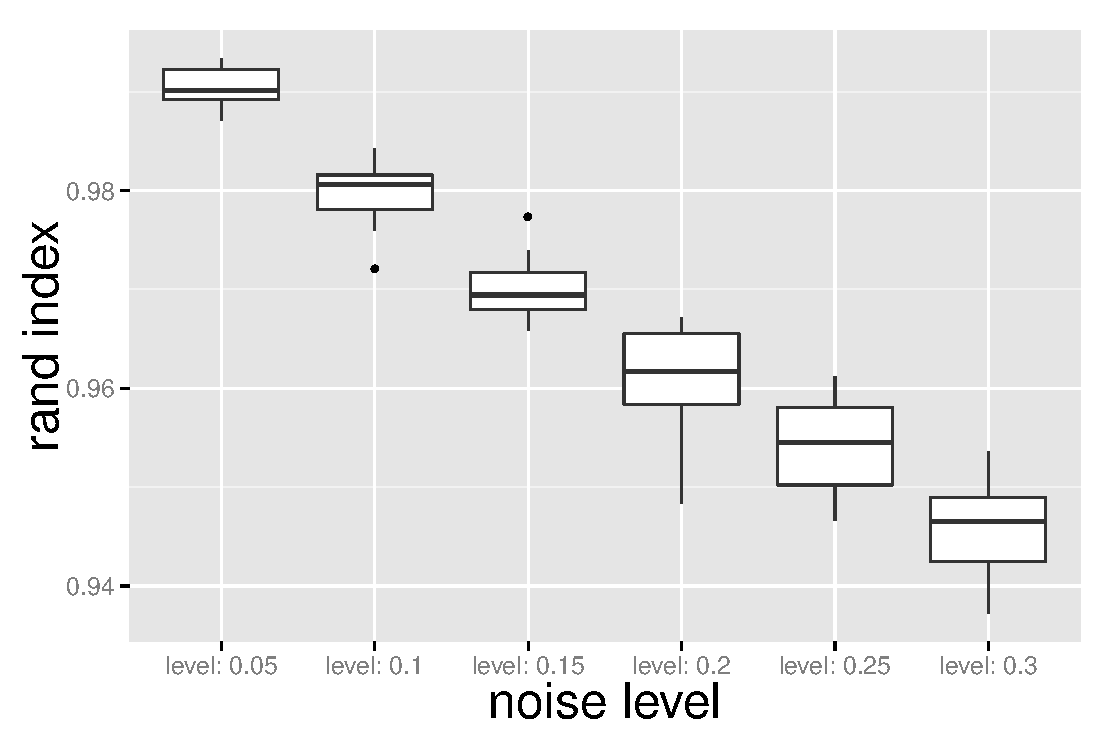
\includegraphics[width=\textwidth,height=0.8\textwidth]{fig/noise_boxplot_col.pdf}
    \subcaption{}
  \end{minipage}
  \begin{minipage}[t]{0.34\textwidth}
    \centering
    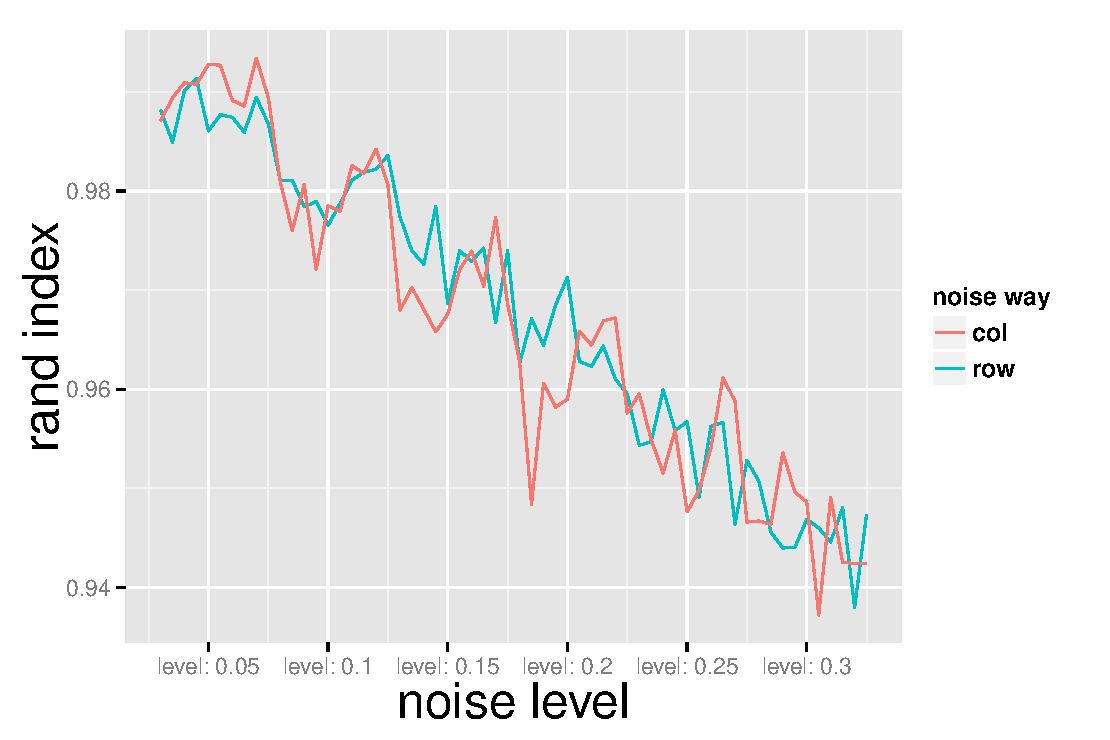
\includegraphics[width=\textwidth,height=0.8\textwidth]{fig/noise_line.pdf}
    \subcaption{}
  \end{minipage}
  \caption{\textbf{\textit{Rand Index} between the clustering of noised data and the raw data.} \textbf{(a)} Noises added on each row. \textbf{(b)}  Noises added on each column. \textbf{(c)}Average \textit{Rand Index} in terms of different levels of noises.}
  \label{fig:perturbation}
\end{figure*}



\section{Conclusion}
\label{sec:conc}

\bibliographystyle{plain}
\bibliography{references}

\section{Appendix}

\begin{figure*}
  \begin{minipage}[t]{0.33\textwidth}
    \centering
    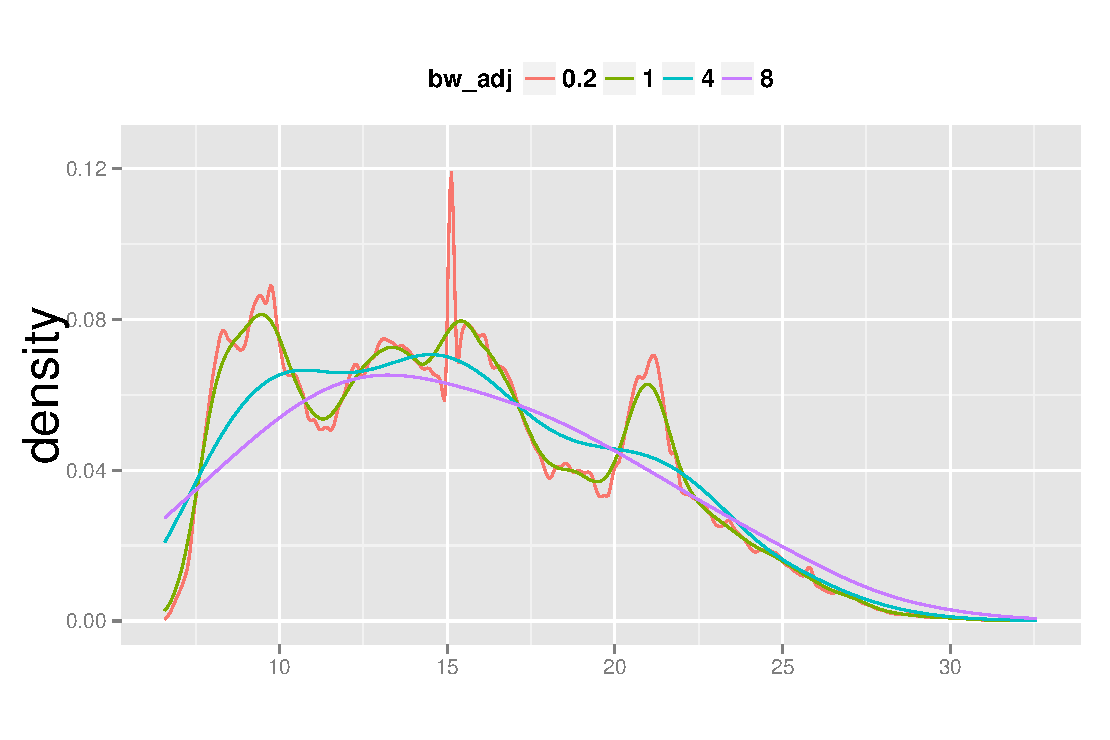
\includegraphics[width=\textwidth,height=\textwidth]{fig/Temperature_biweight.pdf}
    \subcaption{kernel: biweight}
  \end{minipage}
  \begin{minipage}[t]{0.33\textwidth}
    \centering
    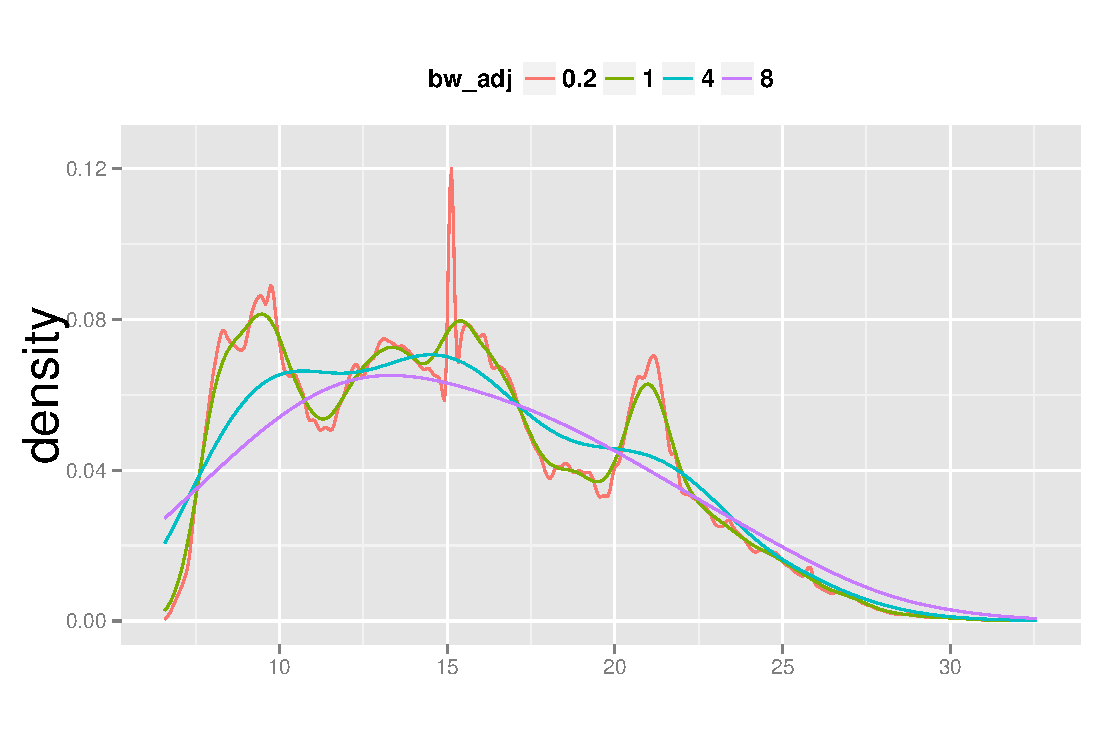
\includegraphics[width=\textwidth,height=\textwidth]{fig/Temperature_cosine.pdf}
    \subcaption{kernel: cosine}
  \end{minipage}
  \begin{minipage}[t]{0.34\textwidth}
    \centering
    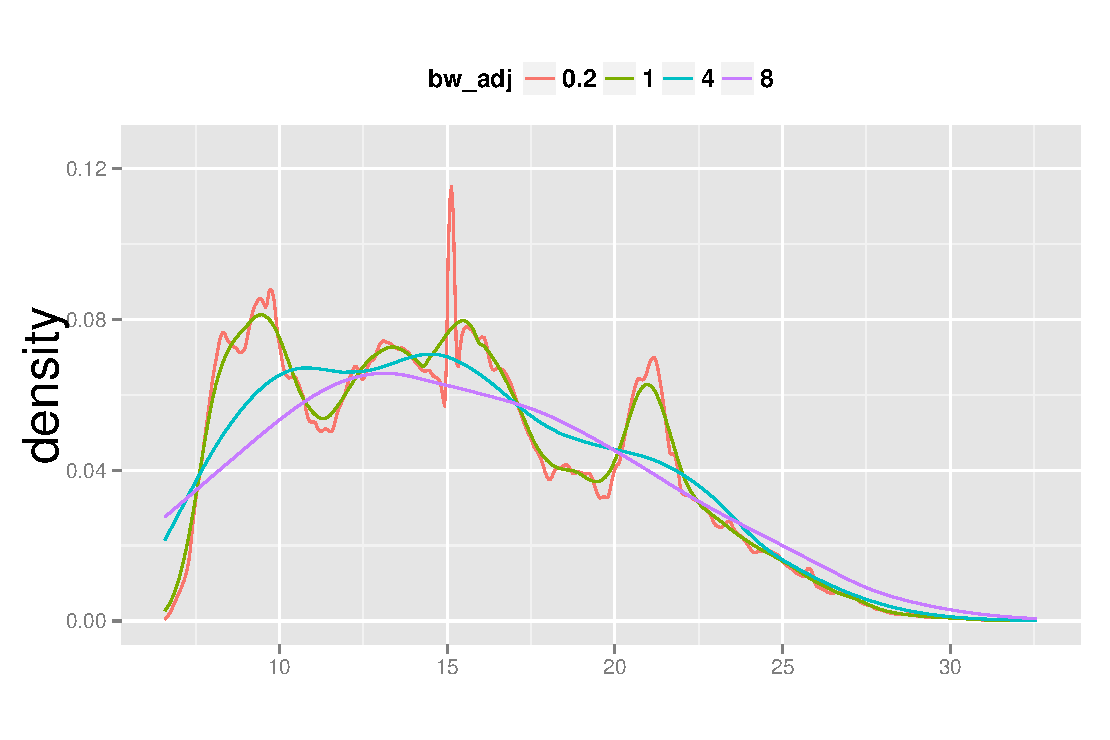
\includegraphics[width=\textwidth,height=\textwidth]{fig/Temperature_epanechnikov.pdf}
    \subcaption{kernel: epanechnikov}
  \end{minipage}\\
    \begin{minipage}[t]{0.33\textwidth}
    \centering
    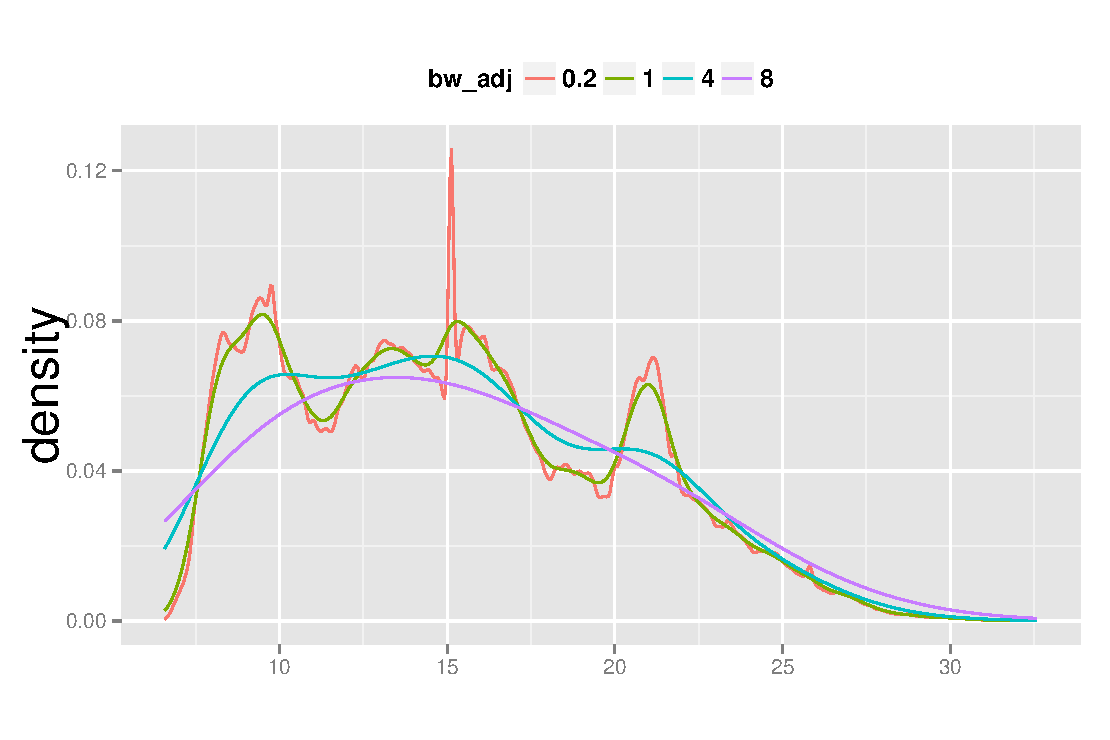
\includegraphics[width=\textwidth,height=\textwidth]{fig/Temperature_Gaussian.pdf}
    \subcaption{kernel: gaussian}
  \end{minipage}
  \begin{minipage}[t]{0.33\textwidth}
    \centering
    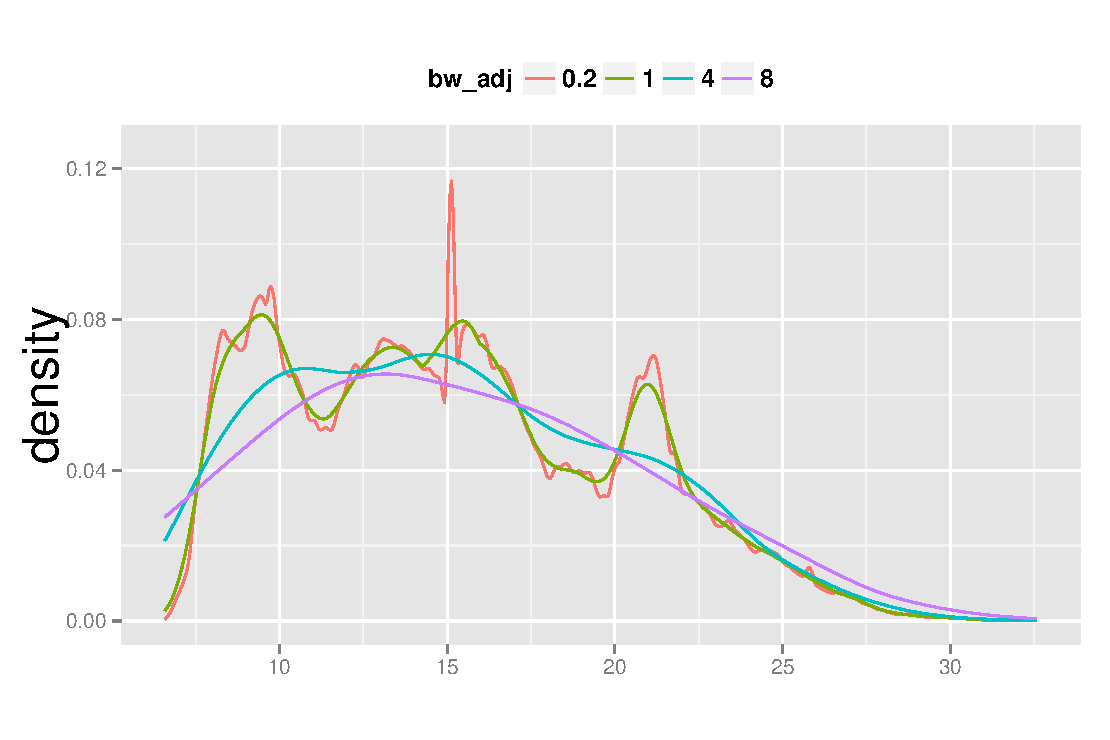
\includegraphics[width=\textwidth,height=\textwidth]{fig/Temperature_optcosine.pdf}
    \subcaption{kernel: optcosine}
  \end{minipage}
  \begin{minipage}[t]{0.34\textwidth}
    \centering
    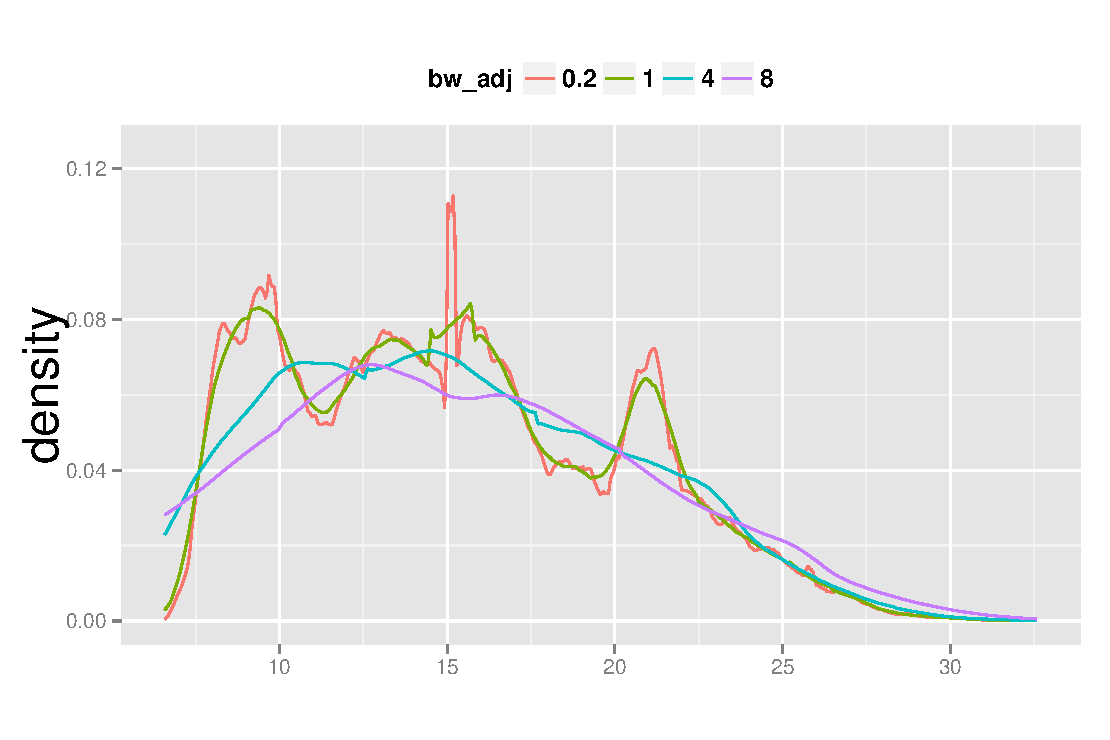
\includegraphics[width=\textwidth,height=\textwidth]{fig/Temperature_rectangular.pdf}
    \subcaption{}
  \end{minipage}\\
  \begin{minipage}[t]{0.33\textwidth}
    \centering
    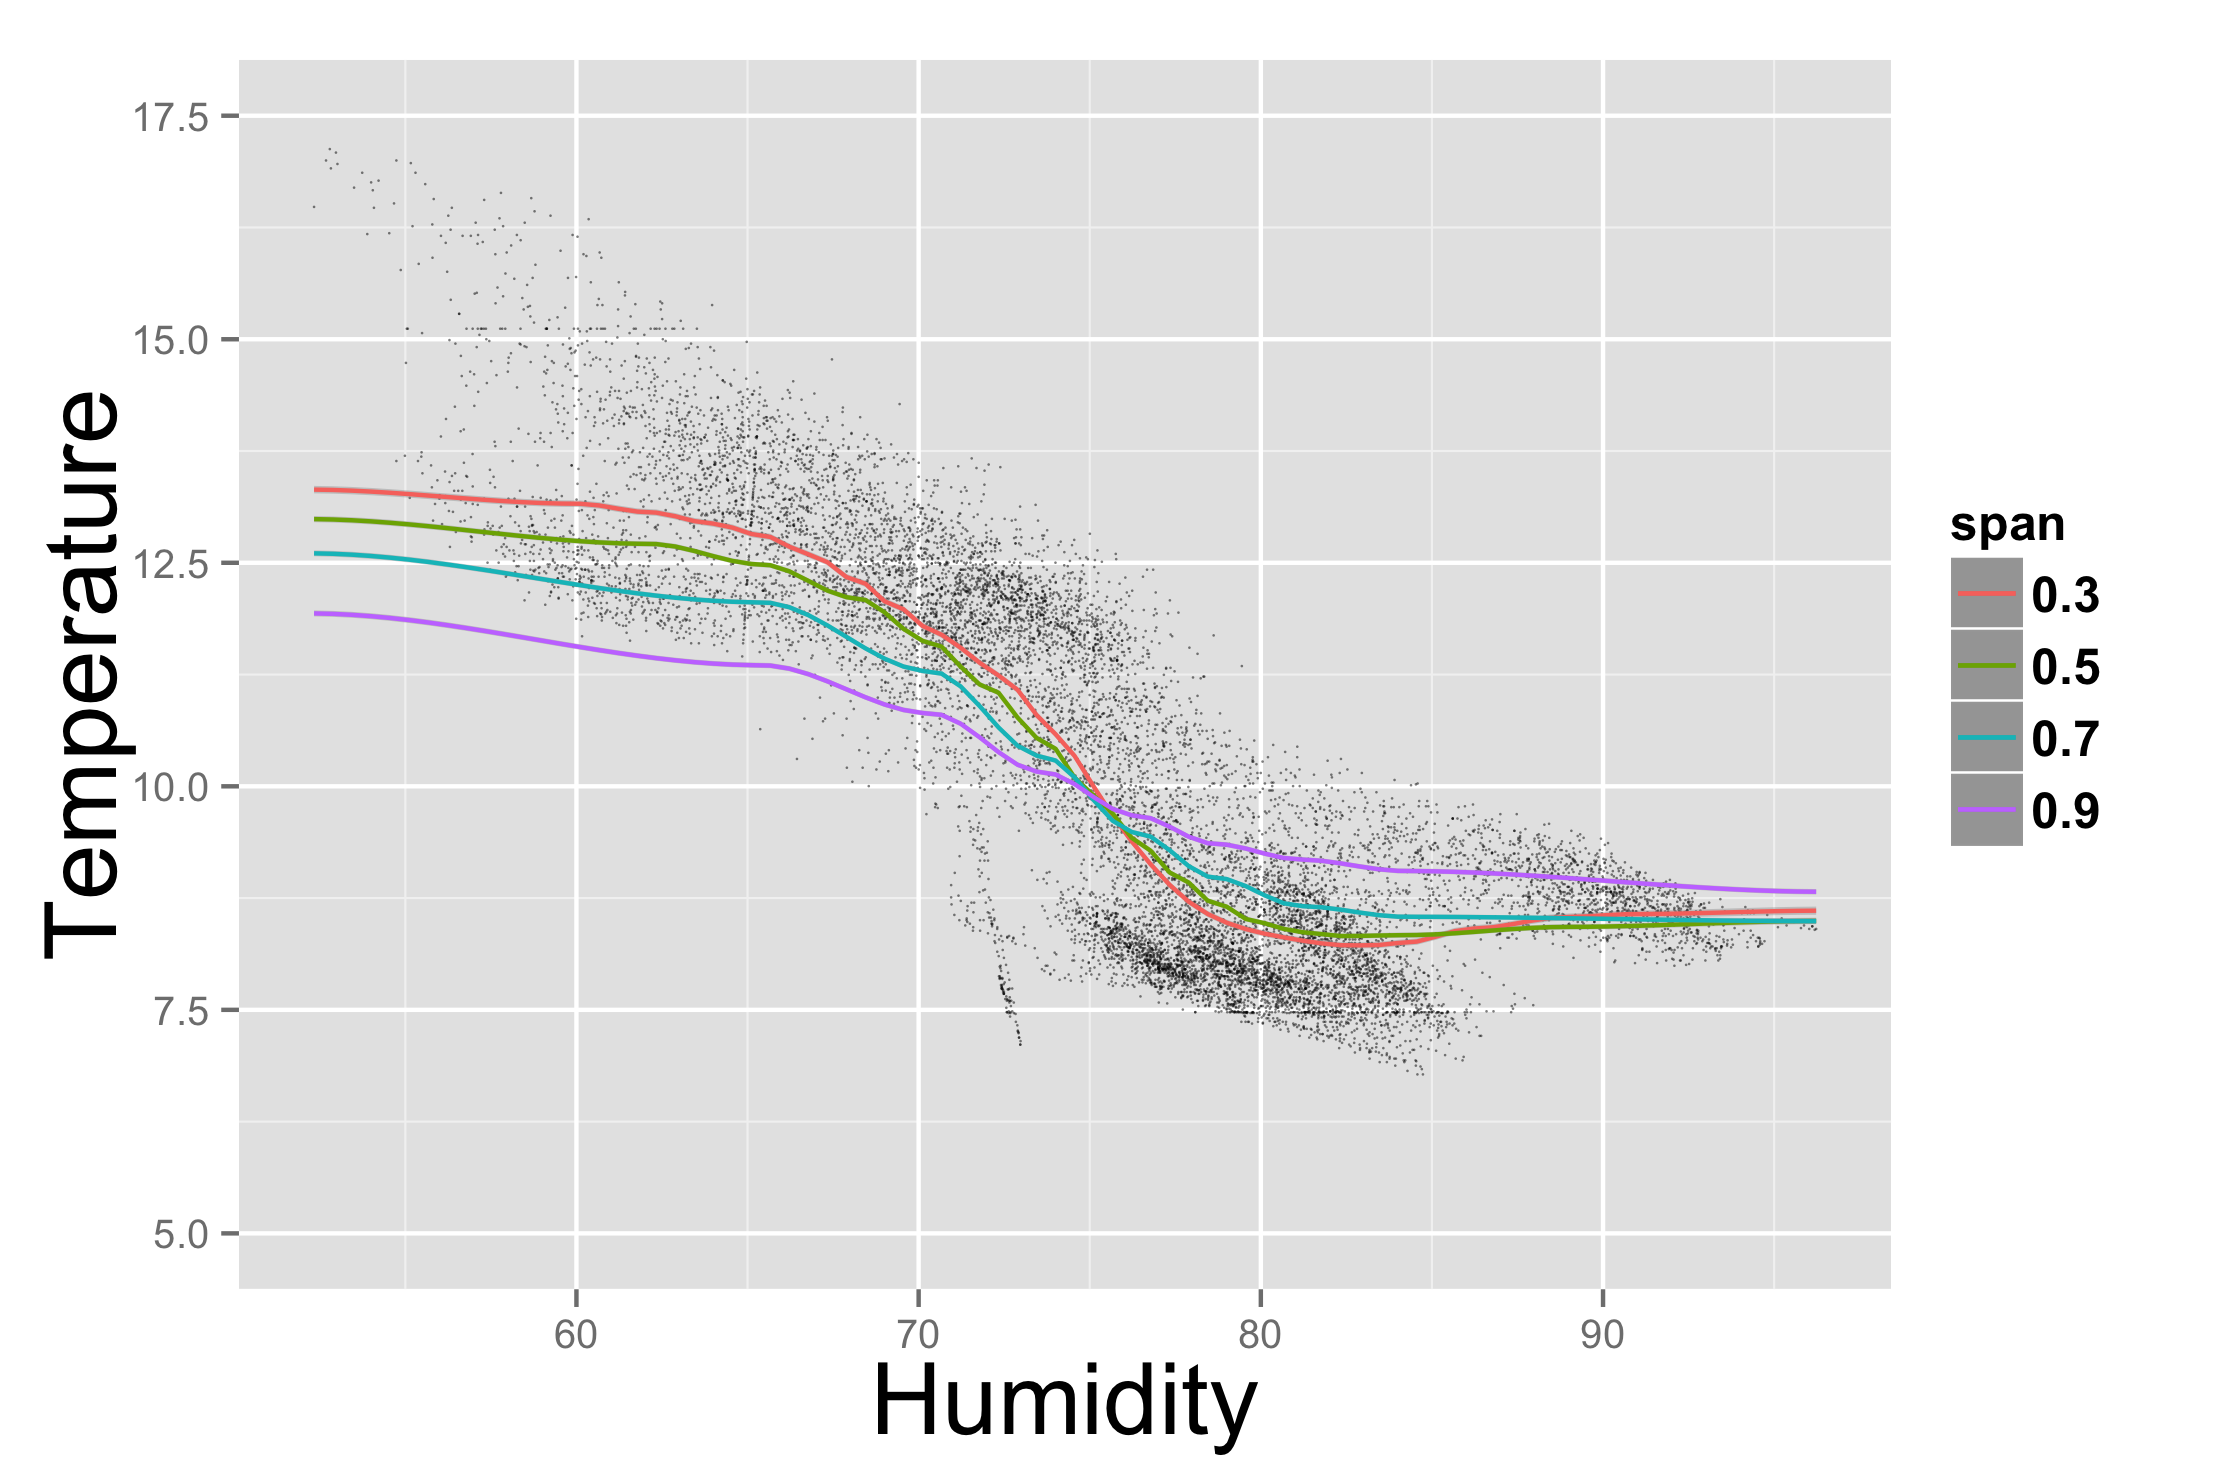
\includegraphics[width=\textwidth,height=\textwidth]{fig/Humid_Temp_Loess_poly0.png}
    \subcaption{degree = 0}
  \end{minipage}
  \begin{minipage}[t]{0.33\textwidth}
    \centering
    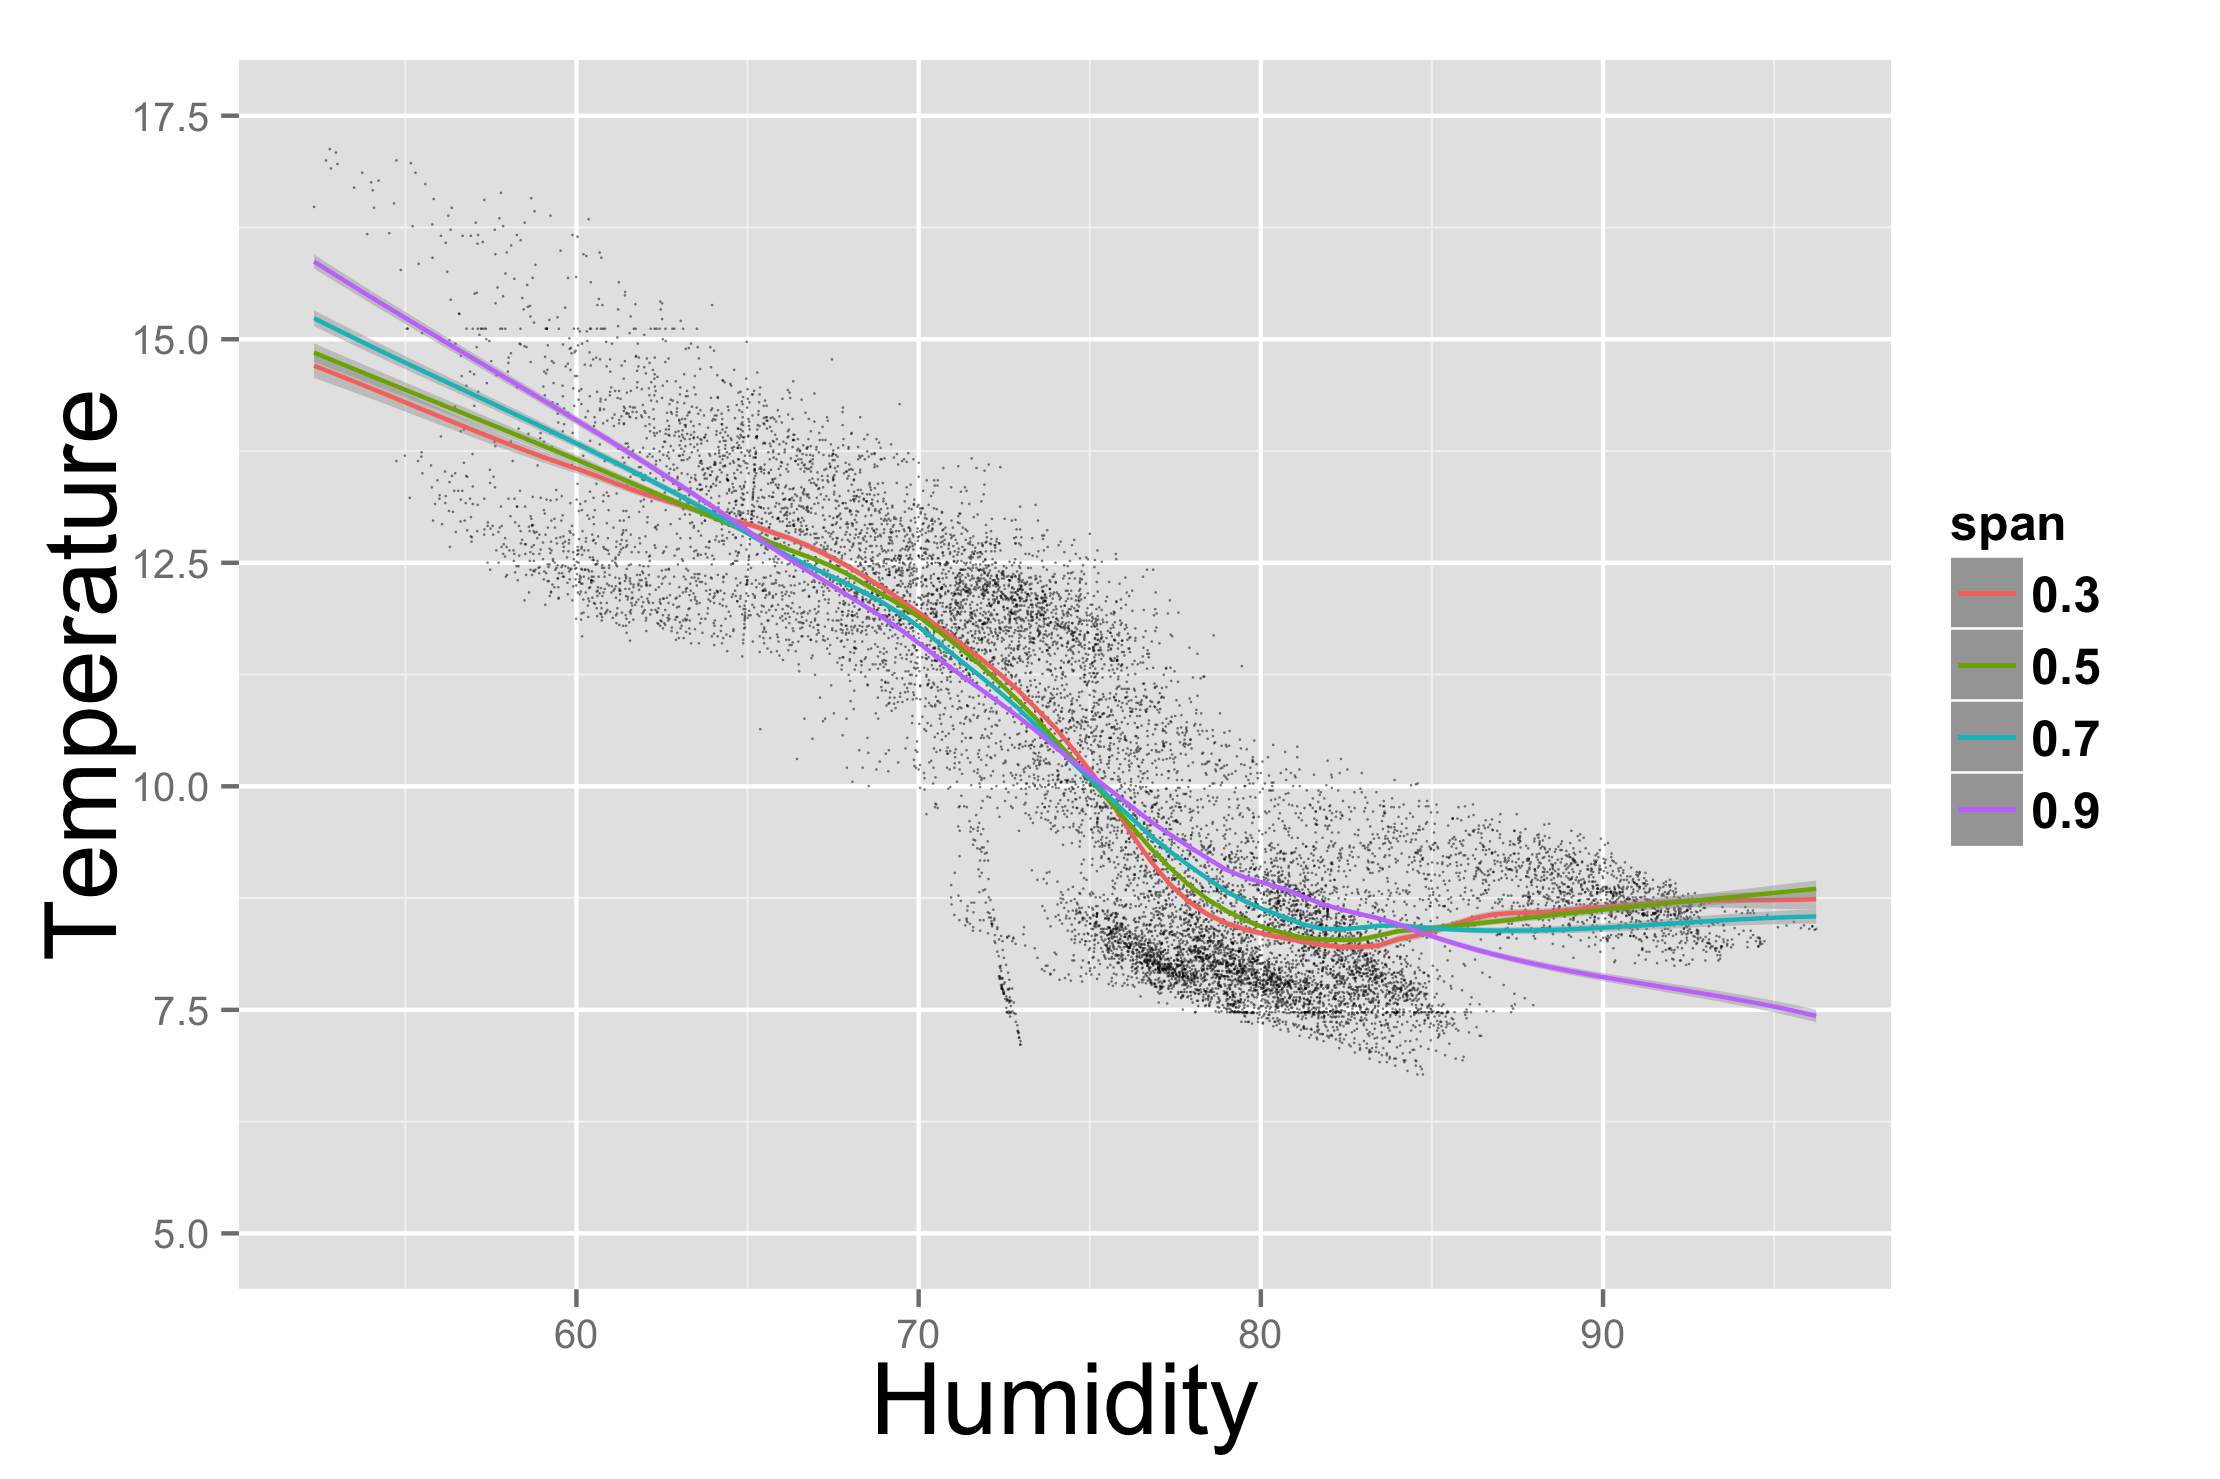
\includegraphics[width=\textwidth,height=\textwidth]{fig/Humid_Temp_Loess_poly1.png}
    \subcaption{degree = 1}
  \end{minipage}
  \begin{minipage}[t]{0.34\textwidth}
    \centering
    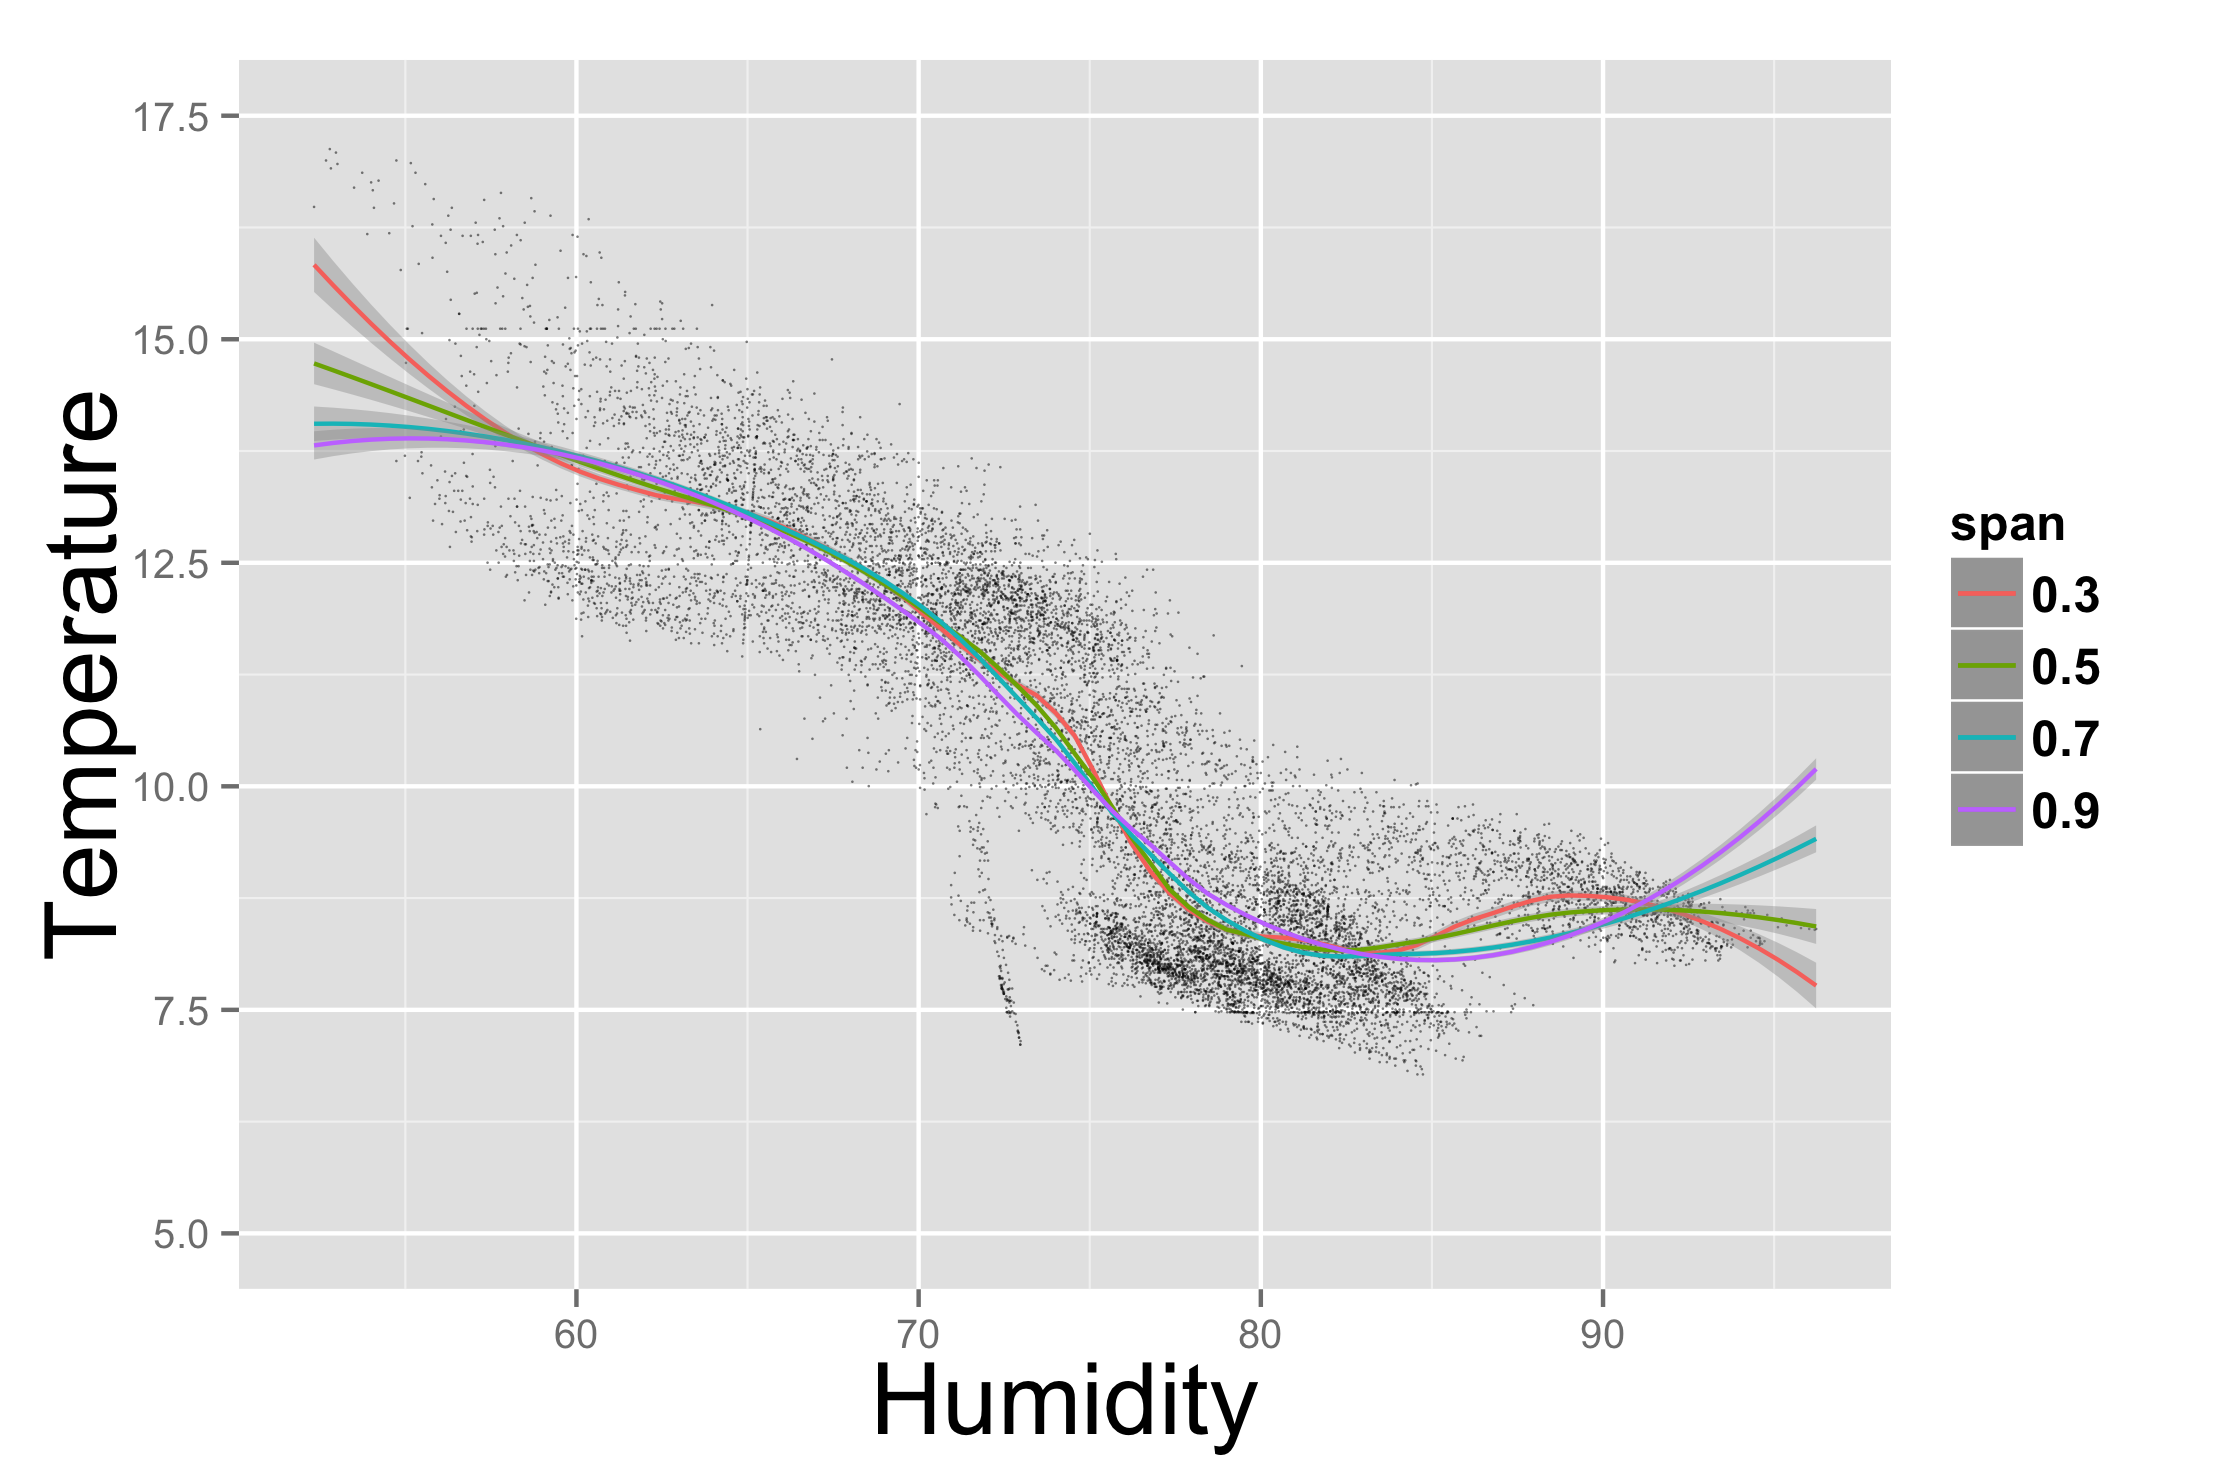
\includegraphics[width=\textwidth,height=\textwidth]{fig/Humid_Temp_Loess_poly2.png}
    \subcaption{degree = 2}
  \end{minipage}\\
  \caption{\textbf{Kernel density and LOESS.}(a)-(f) Kernel density for temperature measurements. (g)-(k) LOESS on the relationship between Temperature and Humidity.}   
  \label{fig:Kernel_LOESS}
\end{figure*}


\end{document}
